         \chapter{Die atoom}\fancyfoot[LO,RE]{Chemistry: Matter and Materials}
\label{chap:atom}
    \setcounter{figure}{1}
    \setcounter{subfigure}{1}
    \label{ea1c9e59656f96ee804546971cf6dee6}
    \label{m38756*cid1}
            \section{Inleiding}
            \nopagebreak
  
      \par \label{m38756*id254141}Ons het nou gekyk na die talle voorbeelde van die tipes materie en materiale wat rondom ons bestaan
en ons het sommige van die maniere waarop materiale geklassifiseer word, ondersoek. Waaruit bestaan hierdie materiale nou eintlik en wat maak een materiaal verskillend van 'n ander? Ten einde hierdie vraag te beantwoord, moet ons die boustene van materie, \textbf{atome}, van naderby bekyk. Atome vorm die basis van al die strukture en organismes in die heelal. Die planete, son, gras, bome, lug wat ons inasem en mense is almal opgebou uit verskillende kombinasies van atome.\par 
            

\chapterstartvideo{P10020}



\begin{project}{Biblioteek-opdrag: Modelle van die atoom}
            \nopagebreak
            \label{m38756*eip-3}

Ons huidige begrip van die atoom het ontwikkel oor 'n lang tydperk met 'n groot groep verskillende mense wat hierin 'n rol gespeel het. Doen 'n bietjie navorsing oor die ontwikkeling van die verskillende idees oor die atoom en die mense wat bygedra het tot hierdie studie. Sommige mense na wie se werk in hierdie verband gekyk kan word, sluit in: JJ Thomson, Ernest Rutherford, Marie Curie, JC Maxwell, Max Planck, Albert Einstein, Niels Bohr, Lucretius, LV de Broglie, CJ Davison, LH Germer, Chadwick, Werner Heisenberg, Max Born, Erwin Schrodinger, John Dalton, Empedocles, Leucippus,
Democritus, Epicurus, Zosimos, Maria die Jodin, Geber, Rhazes, Robert Boyle, Henry Cavendish, A Lavoisier en H Becquerel. Jy hoef nie inligting oor al hierdie mense te soek nie, maar probeer iets kry oor so veel van hulle as moontlik.
\par \begin{minipage}{.5\textwidth}
\label{m38756*id7342}Maak 'n lys van die belangrikste bydraes wat elkeen van hierdie mense gemaak het tot die opbou van 'n model van die atoom en maak dan 'n tydlyn van hier\-die inligting. (Jy kan 'n aanlynhulpmiddel soos Dipity \textsl(http://www.dipity.com/) gebruik om 'n tydlyn te maak.) Probeer om 'n idée te kry hoe alles uiteindelik bymekaar gevoeg is om ons te bring tot by vandag se moderne begrip van die atoom.
\end{minipage}
\begin{minipage}{.5\textwidth}
 \begin{center}
  \includegraphics[width=0.6\textwidth]{photos/timeline_atom.png}
 \end{center}

\end{minipage}

\end{project}
\par \label{m38756*cid2}

\section{Modelle van die atoom}
            \nopagebreak
      \label{m38756*id254164}Dit is belangrik om te besef dat baie van wat ons vandag weet oor die struktuur van atome, ontwikkel het oor 'n lang tydperk. Dit is dikwels hoe wetenskaplike kennis ontwikkel, met een persoon wat voortbou op die idees van iemand anders. Ons gaan kyk hoe ons moderne begrip van die atoom met verloop van tyd ontwikkel het.\par 

\mindsetvid{The origins of atomic theory}{VPakv}

      \label{m38756*id254508}
Die idee van atome is uitgedink deur twee Griekse filosowe, Democritus en Leucippus in die vyfde eeu vC. Die Griekse woord $\alpha \tau o\mu o\nu $ (Atoom) beteken ondeelbaar omdat hulle geglo het dat atome nie in kleiner stukkies gebreek kan word nie.\\
      \label{m38756*id254540}
Vandag weet ons dat atome bestaan uit 'n \textbf{positief} gelaaide kern in die middel omring deur \textbf{negatief gelaaide elektrone}. In die verlede egter, voordat die struktuur van die atoom behoorlik verstaan is, het wetenskaplikes met baie verskillende \textbf{modelle} of \textbf{prente} probeer beskryf hoe atome lyk.

\Definition{Model}{'n Model is 'n voorstelling van 'n stelsel in die werklike wêreld. Modelle help ons om die stelsels en hul eienskappe beter te verstaan. Byvoorbeeld, 'n \textsl{atoommodel} verteenwoordig hoe die struktuur van 'n atoom moontlik \textsl{kan} lyk en is gebaseer op wat ons weet oor die optrede van atome. Dit is nie noodwendig 'n ware beeld van die presiese struktuur van 'n atoom nie.   } 
\subsection*{Dalton se model van die atoom}
\begin{minipage}{.5\textwidth}
John Dalton het voorgestel dat alle materie saamgestel is uit baie klein dele wat hy atome genoem het. Dit was nie 'n totale nuwe konsep nie, aangesien die ou Grieke (veral Democritus) reeds vroeer voorgestel het dat alle materie uit klein, onverdeelbare (kan nie verdeel word nie) eenhede bestaan. Toe Dalton sy model voorgestel het, was die bestaan van iets soos elektrone en die kern nog onbekend. 
\end{minipage}
\begin{minipage}{.5\textwidth}
   \setcounter{subfigure}{0}
	\begin{figure}[H] % horizontal\label{m38756*uid2}
    \begin{center}
\scalebox{.8}{
\begin{pspicture}(-3,-3)(3,3)
%\psgrid[gridcolor=lightgray]
\pscircle(0,0){1}
\end{pspicture}
}
\begin{minipage}{.8\textwidth}
\caption{Die atoom volgens Dalton}
\end{minipage}
\label{fig:atom:dalton}
\end{center}
 \end{figure}
\end{minipage}

      \label{m38756*uid1}
            \subsection*{Thomson se model van die atoom}
            \nopagebreak
\begin{minipage}{.5\textwidth}
        \label{m38756*id254616}
Na afloop van die ontdekking van die elektron deur J.J. Thomson in 1897, het die mense besef dat atome opgebou is uit nog kleiner deeltjies as wat hulle voorheen gedink het. Die atoomkern was egter nog nie ontdek nie en so is die "Pruimpoeding model" voorgestel in 1904. In hierdie model bestaan die atoom uit negatiewe elektrone wat dryf in  'n “sop” van positiewe ladings, baie soos pruime in 'n poeding of rosyne in 'n vrugtekoek (Figuur~\ref{fig:atom:plumpudding}). In 1906 het Thomson die Nobelprys ontvang vir sy werk in hierdie veld. Selfs met die pruimpoeding model was daar nog geen begrip van hoe die elektrone in  'n atoom gerangskik was nie.\\ 
\end{minipage}
\begin{minipage}{.5\textwidth}
    \setcounter{subfigure}{0}
	\begin{figure}[H] % horizontal\label{m38756*uid2}
    \begin{center}
\scalebox{.7}{
\begin{pspicture}(-3,-3)(3,3)
%\psgrid[gridcolor=lightgray]
\psellipse(0,0)(2.5,2.5)
\psline[linewidth=0.3cm](0,2)(0,-2)
\psline[linewidth=0.3cm](-2,0)(2,0)
\psellipse(-1.5,1.5)(0.25,0.25)
\rput(-1.5,1.5){\textbf{-}}
\psellipse(-1,1)(0.25,0.25)
\rput(-1,1){\textbf{-}}
\psellipse(-1.5,-1)(0.25,0.25)
\rput(-1.5,-1){\textbf{-}}
\psellipse(-1,-1.5)(0.25,0.25)
\rput(-1,-1.5){\textbf{-}}
\psellipse(1,1.5)(0.25,0.25)
\rput(1,1.5){\textbf{-}}
\psellipse(1.5,-1.5)(0.25,0.25)
\rput(1.5,-1.5){\textbf{-}}
\psellipse(1,0.5)(0.25,0.25)
\rput(1,0.5){\textbf{-}}
\psellipse(1,-1)(0.25,0.25)
\rput(1,-1){\textbf{-}}
\psline(1.2,1.6)(3,1.6)
\rput(4,1.6){\textbf{electrons}}
\psline(2,-1)(3,-1)
\rput(3.8,-1){\textbf{'soup' of}}
\rput(4.3,-1.5){\textbf{positive charge}}
\end{pspicture}
}
\begin{minipage}{.8\textwidth}
\caption{Die atoom volgens \\ die pruimpoeding-model}
\end{minipage}
\label{fig:atom:plumpudding}
\end{center}
 \end{figure}    
\end{minipage}   
      

\IFact{Twee ander modelle wat voorgestel is vir die atoom, is die kubieke model en die Saturniese model. In die kubieke model is die elektrone voorgestel om hulle te bevind op die hoeke van 'n kubus. In die Saturniese model is daar beskryf dat die elektrone rondom  'n groot, swaar kern sou wentel.}
  
Die ontdekking van \textbf{bestraling} was die volgende stap op die pad na die opbou van 'n akkurate beeld van atoomstruktuur. In die vroe\"{e} twintigste eeu het Marie Curie en haar man, Pierre, ontdek dat sommige elemente (die \textsl{radio-aktiewe elemente}) deeltjies uitstraal wat in staat is om deur materie te dring op soortgelyke wyse as X-strale (Lees meer hieroor in Graad 11). Dit was Ernest Rutherford wat in 1911 hierdie ontdekking gebruik het om die model van die atoom te hersien.\par 
      

      
            \subsection*{Rutherford se model van die atoom}
            \nopagebreak
\begin{minipage}{.5\textwidth}
            \label{m38756*id254751}
Rutherford het eksperimente uitgevoer wat gelei het tot 'n verandering in die idees rondom die atoom. Sy nuwe model het die atoom beskryf as 'n klein, digte, positief- gelaaide sentrale deel wat die kern genoem is en wat omring is deur die ligter, negatief- gelaaide elektrone.  'n
Ander interpretasie van hierdie model was dat die atoom gesien is as 'n mini-sonnestelsel waar die elektrone rondom die kern wentel
soos planete wat om die son draai. 'n Vereenvoudigde prentjie van hierdie model word getoon in Figuur~\ref{fig:atom:rutherfordmodel}. Hierdie model word soms die \textbf{sonnestelsel-model} van die atoom genoem. \par 
\end{minipage}
\begin{minipage}{.5\textwidth}
    \setcounter{subfigure}{0}
	\begin{figure}[H] % horizontal\label{m38756*uid5}
    \begin{center}
\scalebox{.8}{
\begin{pspicture}(-2.2,-2.4)(2.2,2.4)
\SpecialCoor
%\psgrid%[gridcolor=lightgray]
\def\water{\psset{unit=0.2}\rput{150}{\pscircle[fillcolor=white,fillstyle=solid](0,0){2}
\psarc[fillcolor=white,fillstyle=solid](-1.5,1){1.5}{30}{260}
\psarc[fillcolor=white,fillstyle=solid](1.5,1){1.5}{280}{150}
\rput(-1.5,1){\pscurve(1.5;30)(-1;142.5)(1.5;260)}
\rput(1.5,1){\pscurve(1.5;150)(-1;37.5)(1.5;280)}}}

\def\atom{\rput(0,0){\water}\rput{180}(0.25,0.25){\water}\rput{45}(0.25,0.25){\water}\rput{225}(0.25,0.25){\water}}

\rput(0,0){\atom}
\psellipse[linecolor=lightgray,linewidth=3pt](0,0)(1.5,2.2)
\rput{120}{\psellipse[linecolor=lightgray,linewidth=3pt](0,0)(1.5,2.2)}
\rput{240}{\psellipse[linecolor=lightgray,linewidth=3pt](0,0)(1.5,2.2)}

\psdots[dotsize=5pt](1,1.6)(-1,-1.6)\uput[ur](1,1.6){electron orbiting the nucleus}
\rput{120}{\psdots[dotsize=5pt](1,1.6)(-1,-1.6)}
\rput{240}{\psdots[dotsize=5pt](1,1.6)(-1,-1.6)}
\uput[r](2.4,0){nucleus}
\psline{<-}(1,0)(2.4,0)
\end{pspicture}
}
\caption{Rutherford se model van die atoom}
\end{center}
\label{fig:atom:rutherfordmodel}
 \end{figure} 
\end{minipage}      
      \label{m38756*uid6}
            \subsection*{Bohr se model van die atoom}
            \nopagebreak
\begin{minipage}{.5\textwidth}
        \label{m38756*id254784}
Daar was egter 'n paar probleme met Rutherford se model: dit kon byvoorbeeld nie die interessante waarneming verklaar dat atome slegs lig uitstraal by sekere golflengtes of frekwensies nie. Niels Bohr het hierdie probleem opgelos deur voor te stel dat die elektrone rondom die kern wentel in sekere spesiale bane by verskillende energievlakke.\par 
\end{minipage}
\begin{minipage}{.5\textwidth}
   \setcounter{subfigure}{0}
	\begin{figure}[H] % horizontal\label{m38756*uid2}
    \begin{center}
\scalebox{.5}{
\begin{pspicture}(-6,-6)(6,6)
%\psgrid[gridcolor=lightgray]
\pscircle[fillstyle=solid,fillcolor=gray](0,0){0.1}
\pscircle[linecolor=darkgray,linewidth=0.1](0,0){1}
\pscircle[linecolor=darkgray,linewidth=0.1](0,0){2}
\pscircle[linecolor=darkgray,linewidth=0.1](0,0){3}
\psline[linewidth=0.05]{<-}(0.1,0)(4,0)
\uput[r](4,0){\Large{nucleus}}
\psline[linewidth=0.05]{<-}(1.8,1)(4,1)
\uput[r](4,1){\Large{electron orbit}}
\end{pspicture}
}
\begin{minipage}{.8\textwidth}
\caption{Bohr se model van die atoom}
\end{minipage}
\label{fig:atom:dalton}
\end{center}
 \end{figure}
\end{minipage}

\label{m38756*notfhsst!!!underscore!!!id119}
\subsection*{James Chadwick}
Rutherford het voorspel (in 1920) dat 'n ander soort deeltjie saam met die proton teenwoordig moet wees in die kern. Hy het hierdie voorspelling gemaak op grond van die feit dat as daar slegs positief- gelaaide protone in die kern was, dit uitmekaar sou breek as gevolg van die afstotende kragte tussen die soortgelyke ladings van die protone! Om te verseker dat die atoom elektries neutraal bly, moes hierdie deeltjies self neutraal wees. In 1932 het James Chadwick die neutron ontdek en sy massa bepaal.
\label{m38756*eip-279}
            \subsection*{Ander modelle van die atoom}
            \nopagebreak
            \label{m38756*eip-993}
Alhoewel die mees algemene model van die atoom die Bohr-model is, is wetenskaplikes nogsteeds besig om nuwe en verbeterde teorieë te ontwikkel oor die bou van die atoom. Een van die belangrikste bydraes tot atoomteorie (die wetenskaplike studie van atome) was die ontwikkeling van kwantumteorie. Schrödinger, Heisenberg, Born en baie ander het 'n rol gespeel in die ontwikkeling van kwantumteorie. 
\par \label{m38756*eip-179}
            \begin{exercises}{Modelle van die atoom}
{
            \nopagebreak
            \label{m38756*eip-786}Pas die inligting in Kolom A by die belangrikste ontdekker in kolom B.
    % \textbf{m38756*eip-551}\par
          \begin{table}[H]
    % \begin{table}[H]
    % \\ '' '0'
        \begin{center}
      \label{m38756*eip-551}
      \begin{tabular}{|l|l|}\hline
        Kolom A &
        Kolom B \\ \hline
        Ontdekking van elektrone en die pruimpoeding-model & Niels Bohr \\ \hline
        Rangskikking van elektrone & Marie en Pierre Curie  \\ \hline
        AAtome as die kleinste boustene van materie & Antieke Grieke \\ \hline
        Die ontdekking van die kern & JJ Thomson \\ \hline
        Die ontdekking van bestraling & Rutherford \\ \hline
    \end{tabular}
      \end{center}
\end{table}

\practiceinfo
 \par \begin{tabular}[h]{cccccc}
 (1.) l4g  &
\end{tabular}
}
\end{exercises}

            \section{Atoommassa en deursnee}
            \nopagebreak
            \label{m38756*id254850}Dit is soms moeilik om 'n begrip te vorm van die grootte of massa van 'n atoom , want ons kan nie  'n atoom sien nie en ons is ook nie gewoond daaraan om te werk met sulke klein metings nie.\par 
      \label{m38756*uid7}
            \subsection*{Hoe swaar is 'n atoom?}
            \nopagebreak
        \label{m38756*id254863}
Dit is moontlik om die massa van 'n enkele atoom in kilogram te bepaal. Om dit te doen, benodig jy spesiale instrumente en die waardes wat jy sou kry, sou baie lomp wees en ook moeilik om mee te werk. Die massa van 'n koolstofatoom, byvoorbeeld, is ongeveer  $1,99\ensuremath{\times}{10}^{-26}\phantom{\rule{2pt}{0ex}}\text{kg}$, terwyl die massa van 'n atoom waterstof ongeveer $1,67\ensuremath{\times}{10}^{-27}\phantom{\rule{2pt}{0ex}}\text{kg}$ is. As 'n mens kyk na hierdie baie klein getalletjies, is dit nogal baie moeilik om  'n vergelyking te tref tussen die massas van verskillende atome.\par 
        \label{m38756*id254908}
Om die situasie makliker te maak, gebruik wetenskaplikes 'n ander eenheid vir massa wanneer hulle die massa van  'n atoom beskryf. Hierdie eenheid staan bekend as \textbf{atoommassa-eenhede} (ame). Ons kan hierdie eenheid afkort (verkort) tot slegs "u". Wetenskaplikes gebruik die \textbf{koolstof standaard} om ame te bepaal. Die koolstof-standaard gee koolstof 'n atoommassa van 12 u. In vergelyking met koolstof, sal die massa van 'n waterstofatoom slegs 1 u wees. Jy kan dit kontroleer deur die massa van 'n koolstofatoom in kilogram (sien hierbo) te deel deur deur die massa van 'n waterstofatoom in kilogram (jy sal beslis  'n sakrekenaar hiervoor nodig hê!). As jy die berekening doen, sal jy sien dat die massa van 'n
koolstofatoom twaalf keer groter is as die massa van 'n waterstofatoom. Wanneer ons atoommassa-eenhede gebruik in plaas van kilogram, is dit makliker is om dit raak te sien. Atoommassa-eenhede gee ons dus nie die werklike massa van 'n atoom nie, maar eerder die massa met betrekking tot die massa van een (spesifiek uitgesoekte) atoom in die Periodieke Tabel. Met ander woorde, dit is slegs 'n syfer in vergelyking met 'n ander syfer. Die belangrikste aspek om hier te onthou, is dat die atoommassa-eenheid relatief is met betrekking tot een (spesifiek uitgesoekte) element. Die atoommassas van sommige elemente word in Tabel~\ref{tab:atomic mass} aangetoon.
    % \textbf{m38756*uid8}\par
          \begin{table}[H]
    % \begin{table}[H]
    % \\ '' '0'
        \begin{center}
      \label{m38756*uid8}
    \noindent
      \begin{tabular}{|l|l|}\hline
                  \textbf{Element}
                 &
                  \textbf{Atoommassa (u)}
                \\ \hline
        Koolstof ($\text{C}$) &
        12 \\ \hline
        Stikstof ($\text{N}$) &
        14 \\ \hline
        Broom ($\text{Br}$) &
        80 \\ \hline
        Magnesium ($\text{Mg}$) &
        24 \\ \hline
        Kalium ($\text{K}$) &
        39 \\ \hline
        Kalsium ($\text{Ca}$) &
        40 \\ \hline
        Suurstof ($\text{O}$) &
        16 \\ \hline
    \end{tabular}
      \end{center}
    \caption{Die atoommassagetal van 'n paar van die elemente.}
\label{tab:atomic mass}
\end{table}
    \par
        \label{m38756*id255096}
Die werklike waarde van 1 atoommassa-eenheid is $1,67\ensuremath{\times}{10}^{-24}\phantom{\rule{2pt}{0ex}}\text{g}$ of $1,67\ensuremath{\times}{10}^{-27}\phantom{\rule{2pt}{0ex}}\text{kg}$. Dis 'n baie klein massa! As ons dit uitskryf, lyk dit soos volg: $0,000~000~000~000~000~000~000~000~167~\text{kg}$. 'n Atoom is dus baie, baie klein.\par 
\label{m38756*eip-320}
            \subsection*{Rutherford se alfadeeltjie verstrooiing eksperiment}
            \nopagebreak
            \label{m38756*id254668}
Radioaktiewe elemente straal verskillende soorte deeltjies uit. Sommige van hierdie deeltjies is positief gelaaide alfa ($\alpha $) deeltjies. Rutherford wou uitvind waar presies die positiewe lading in 'n atoom is. Hy het  'n reeks eksperimente uitgevoer waar hy velle bladgoud met alfapartikels bombardeer het.  'n Vereenvoudigde diagram van sy eksperiment word in figuur~\ref{fig:atom:goldfoil} aangetoon.\par 

\begin{figure}[H] % horizontal\label{m38756*uid4}
 \begin{center}
\scalebox{.8}{
\begin{pspicture}(-4,-3)(9,3)
\SpecialCoor
%\psgrid%[gridcolor=lightgray]

\def\gold{\pscircle(0,0){0.2}\psdot(0,0)}

\rput(0,0){
\psarc[linewidth=2pt](0,0){3}{270}{90}
\psframe[fillcolor=lightgray,fillstyle=solid](-0.2,-2)(0,2)
\psframe[fillcolor=white,fillstyle=solid](-4,-0.5)(-2,0.5)
\rput(-3,0.2){radioactive}
\uput[d](-3,0.2){substance}
\psline[linewidth=1.5pt]{->}(-2,0)(-0.2,0)
\uput[d](-1.1,0){$\alpha$ particles}
\psline[linestyle=dashed](-0.2,0)(-2,3)
\uput[dr](-1.8,3){C}
\psline[linestyle=dashed](-0.2,0)(-2,-3)
\uput[ur](-1.8,-3){C}

\psline[linestyle=dashed](0,0)(2,2.2)
\uput[l](2,2.2){B}
\psline[linestyle=dashed](0,0)(2,-2.2)
\uput[l](2,-2.2){B}

\psline[linestyle=dashed](0,0)(3,0)
\psline[linestyle=dashed](0,0)(3,0.2)
\uput[ul](3,0.2){A}
\psline[linestyle=dashed](0,0)(3,-0.2)
\uput[dl](3,-0.2){A}

\uput[ur](1.3,-3){Zinc Sulfide screen}}

\rput(5,0){
\psframe(0,-2)(1,2)
\multirput(0.2,-1.8)(0,0.4){10}{\gold}
\multirput(0.5,-1.6)(0,0.4){9}{\gold}
\multirput(0.8,-1.8)(0,0.4){10}{\gold}

\psline{->}(-1,1.5)(2,1.5)\uput[ul](2,1.5){A}
\psline{->}(-1,0.35)(0.5,0.35)(2,0)\uput[ul](2,0){B}
\psline{->}(-1,-1)(0.2,-1)(-1,-2)\uput[u](-1,-2){C}
\pcline[linestyle=none](-1,-2)(-1,2)
\lput*{:U}{$\alpha$ particles}
\psline(0.8,-1.4)(1.4,-1.4)
\rput[l](1.4,-1.4){nucleus of}
\uput[dr](1.4,-1.5){gold atom}

}
\rput(-3,-2.5){(a)}
\rput(5.5,-2.5){(b)}
\psline(-0.2,1.5)(-2,1.5)
\rput(-3,1.5){gold sheet}
\end{pspicture}
}
\caption{Rutherford se goudblad eksperiment. Figuur (a) toon die pad van die $\alpha$ deeltjies nadat hulle die goudblad getref het. Figuur (b) toon die rangskikking van atome in die goudblad en die pad wat die verskillende $\alpha$ deeltjies volg met betrekking tot die goudblad-atome.}
\label{fig:atom:goldfoil}
\end{center}
\end{figure}       

\mindsetvid{the rutherford model}{VPald}      


Rutherford het sy eksperiment so opgestel dat 'n straal van alfa-partikels gerig was op die goudblaaie. Agter die goudblaaie was 'n skerm gemaak van sinksulfied. Hierdie skerm het Rutherford in staat gestel om te sien waar die alfa-partikels beland het. Rutherford het geweet dat die elektrone in die goud atome nie regtig enige invloed op die pad van die alfa-partikels sou uitoefen nie, omdat die massa van 'n elektron soveel kleiner is as dié van 'n proton. Hy het geredeneer dat dit die positief gelaaide protone sou wees wat die positief gelaaide alfa- partikels sal wegstoot en sodoende hul rigting kan verander.\par 

Wat het hy ontdek het, was dat die meeste van die alfa-partikels ongestoord deur die foelie beweeg het en opgespoor kon word op die skerm direk agter die foelie (A). Sommige van die partikels word effens gedeflekteer na ander dele van die skerm (B). Wat nog meer interessant is, is dat sommige van die deeltjies reguit terug gedeflekteer word in die rigting van waar hulle gekom het (C)! Dit was die deeltjies wat deur die positiewe protone in die goud atome afgestoot is. As die pruimpoeding- model van die atoom waar was, sou Rutherford verwag dat baie meer afstoting sou plaasvind, aangesien die positiewe ladings volgens hierdie model verspreid is oor die hele atoom. Maar dit was nie die geval nie. Die feit dat die meeste deeltjies ongestoord deurbeweeg het, het aangedui dat die positiewe lading slegs gekonsentreer is in een deel van die atoom.\par 

Deur middel van hierdie eksperiment het hy tot die gevolgtrekking gekom dat die kern van die atoom positief gelaai is en gele\"{e} is in die middel van die atoom.
\subsection*{Hoe klein is die kern?}
\begin{minipage}{.5\textwidth}
Die kern van 'n atoom is baie klein. Ons kan die atoom vergelyk met 'n sokkerstadion. As die hele atoom so groot is soos 'n stadion, sal die kern net die grootte van 'n ertjie in die middel van die stadion wees! Dit behoort duidelik te wees dat die atoom hoofsaaklik bestaan uit  'n leë ruimte. As jy al die leë ruimtes verwyder uit die atome in jou liggaam, sou jy die grootte wees van 'n korreltjie sout!
\end{minipage}
\begin{minipage}{.5\textwidth}
\begin{center}
 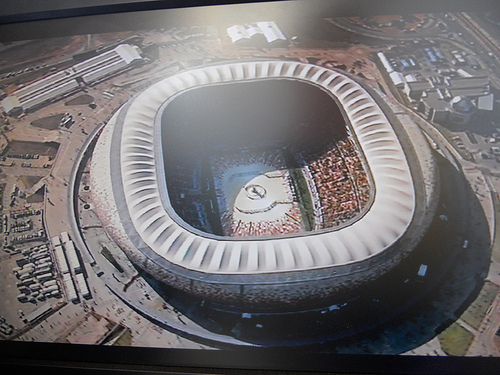
\includegraphics[width=.4\textwidth]{photos/stadiumby-shine2010-flickr.jpg}\par
\textit{Picture by Shine 2010 on Flickr.com}
\end{center}
\end{minipage}
      
            \subsection*{Relatiewe atoommassa}
            \nopagebreak
            \par

\Definition{Relatiewe atoommassa} {Relatiewe atoommassa is die gemiddelde massa van een atoom van al die isotope van  'n spesifieke chemiese element wat natuurlik voorkom, uitgedruk in atoommassa-eenhede.} 


Die relatiewe atoommassa van 'n element is 'n syfer wat jy op die periodieke tabel sal vind. \par 
  


\section{Struktuur van die atoom}
\nopagebreak
\label{m38745*id255206}
As 'n gevolg van die werk wat gedoen is deur vorige wetenskaplikes op atoommodelle (wat ons bespreek het in "modelle van die atoom”), het wetenskaplikes nou 'n goeie idee hoe 'n atoom lyk. Hierdie kennis is belangrik omdat dit ons help om te verstaan ​waarom materie verskillende eienskappe het en waarom sekere materiale met ander verbind. Kom ons bekyk nou die mikroskopiese struktuur van die atoom van naderby. (Hoe die atoom van binne lyk.) \par 

\mindsetvid{the nucleus}{VPaln}

Tot dusver het ons bespreek dat atome bestaan uit 'n positief gelaaide \textbf{kern}, omring deur een of meer negatief gelaaide \textbf{elektrone}. Hierdie elektrone wentel rondom die kern. \par 
      
Voordat ons kyk na 'n paar bruikbare begrippe, moet ons eers verstaan wat elektrone, protone en neutrone is.\par
 
\subsection*{Die Elektron}
\nopagebreak
\label{m38745*id255241}
Die elektron is 'n baie klein deeltjie. Dit het 'n massa van $9,11\ensuremath{\times}{10}^{-31}\phantom{\rule{2pt}{0ex}}\text{kg}$. Wetenskaplikes glo dat die elektron hanteer kan word as \textbf{ 'n deeltjie} of \textbf{element\^{e}re deeltjie} wat beteken dat dit nie opgebreek kan word tot iets kleiner nie. Die elektron dra ook 'n enkele eenheid \textbf{negatiewe} elektriese lading.\par 
\label{m38745*eip-222}
Wat gebeur as 'n atoom elektrone bykry of verloor? Beteken dit dat die atoom nogsteeds deel sal wees van dieselfde element? 'n Verandering in die aantal elektrone van 'n atoom maak nie  'n verskil aan die soort atoom wat dit is nie. Dit sal egter die lading van die atoom verander. Die \textsl{neutraliteit} van die atoom sal verander. As elektrone \textsl{bygevoeg} word, dan word die atoom meer \textsl{negatief} gelaai. Indien elektrone \textsl{weggeneem} word, dan word die atoom meer \textsl{positief} gelaai. Die atoom wat gevorm word in altwee van hierdie gevalle word 'n \textsl{ioon} genoem. 'n Ioon is 'n gelaaide atoom. Byvoorbeeld: 'n neutrale natriumatoom kan 'n elektron verloor en word dan 'n positief gelaaide natriumioon ($\text{Na}^{+}$). 'n Neutrale chlooratoom kan een elektron bykry om 'n negatief gelaaide chloorioon ($\text{Cl}^{-}$) te vorm.\par 


      
\subsection*{Die Kern}
\nopagebreak
\label{m38745*id255305}
In teenstelling met die elektron, \textbf{kan} die kern verdeel word in kleiner boustene naamlik \textbf{protone} en \textbf{neutrone}. Saam word die protone en neutrone \textbf{nukleone} genoem.\par 
        
\subsubsection*{Die Proton}
\nopagebreak
\label{m38745*id255338}
Elke proton dra een eenheid \textbf{positiewe} elektriese lading. Omdat ons weet dat atome \textbf{elektries neutraal} is, m.a.w. dat hulle geen ekstra lading dra nie, moet die aantal protone in 'n atoom dieselfde wees as die aantal elektrone, sodat die positiewe en negatiewe ladings mekaar uitkanselleer. Die totale positiewe lading van 'n kern is gelyk aan die aantal protone in die kern. Die proton is baie swaarder as die elektron (10 000 keer swaarder!) en het 'n massa van $1,6726\ensuremath{\times}{10}^{-27}\phantom{\rule{2pt}{0ex}}\text{kg}$. Wanneer ons praat oor die atoommassa van 'n atoom, word meestal verwys na die gesamentlike massa van die protone en neutrone, dit wil s\^{e}, die nukleone.\par 

        
\subsubsection*{Die Neutron}
\nopagebreak
\label{m38745*id254468}
Die neutron is elektries neutraal, dit wil s\^{e}, dit dra geen lading nie. Soos die proton, is dit baie swaarder as die elektron en die massa is $1,6749\ensuremath{\times}{10}^{-27}\phantom{\rule{2pt}{0ex}}\text{kg}$ (effens swaarder as die proton).\par 
\label{m38745*notfhsst!!!underscore!!!id214}
    % \textbf{m38745*uid14}\par
          \begin{table}[H]
    % \begin{table}[H]
    % \\ '' '0'
        \begin{center}
      \label{m38745*uid14}
    \noindent
      \begin{tabular}{|l|l|l|l|}\hline
         &
                    \textbf{proton}
                   &
                    \textbf{neutron}
                   &
                    \textbf{elektron} \\ \hline
                    \textbf{Massa (kg)}
                   &
        $1,6726\ensuremath{\times}{10}^{-27}$ &
        $1,6749\ensuremath{\times}{10}^{-27}$ &
        $9,11\ensuremath{\times}{10}^{-31}$ \\ \hline
                    \textbf{Eenhede van lading}
                   &
        $+1$ &
        $0$ &
        $-1$ \\ \hline
                    \textbf{Lading(C)}
                   &
        $1,6\ensuremath{\times}{10}^{-19}$ &
        $0$ &
        $-1,6\ensuremath{\times}{10}^{-19}$ \\ \hline
    \end{tabular}
      \end{center}
    \caption{Opsomming van die deeltjies binne die atoom}
\end{table}
    \par

    
\subsection*{Atoomgetal en atoommassagetal}
\nopagebreak
\label{m38745*id255805}
Die chemiese eienskappe van 'n element word bepaal deur die lading van die kern, dit wil sê deur die \textbf{aantal protone}. Hierdie getal word die \textbf{atoomgetal} genoem en word aangedui deur die letter \textbf{Z}.\par 


\Definition{ Atoomgetal (Z)} {Die aantal protone in 'n atoom } 
      
Jy kan die atoomgetal op die periodieke tabel kry. Die atoomgetal is 'n heelgetal en wissel van 1 tot ongeveer 118.\par 
Die massa van 'n atoom hang af van hoeveel nukleone sy kern bevat. Die aantal nukleone, d.w.s. die totale aantal protone \textbf{plus} neutrone, staan bekend as die \textbf{atoommassagetal} en word aangedui deur die letter \textbf{A}. \par 

\Definition{Atoommassagetal (A)} {Die aantal protone en neutrone in die kern van 'n atoom} 

Die atoomgetal (Z) en die massagetal (A) word aangedui deur gebruik van 'n standaardnotasie, byvoorbeeld, koolstof sal soos volg lyk: $_{6}^{12}\text{C}$.

Standaardnotasie toon die chemiese simbool, die atoommassagetal en die atoomgetal van 'n element as volg:\par 
      
    \setcounter{subfigure}{0}
	\begin{figure}[H] % horizontal\label{m38753*id255893}
    \begin{center}
\scalebox{1} % Change this value to rescale the drawing.
{
\begin{pspicture}(0,-1.2192708)(8.541979,1.2192708)
\usefont{T1}{ptm}{m}{n}
\rput(4.2689586,-0.0765625){\Large $^A_Z$}
\usefont{T1}{ptm}{m}{n}
\rput(4.6527085,-0.0965625){\LARGE $X$}
\psline[linewidth=0.02cm,arrowsize=0.113cm 2.5,arrowlength=1.4,arrowinset=0.0]{->}(3.203646,0.8034375)(4.1636457,0.1034375)
\psline[linewidth=0.02cm,arrowsize=0.113cm 2.5,arrowlength=1.4,arrowinset=0.0]{->}(3.203646,-0.8965625)(4.083646,-0.4165625)
\psline[linewidth=0.02cm,arrowsize=0.113cm 2.5,arrowlength=1.4,arrowinset=0.0]{<-}(4.923646,-0.1165625)(5.8036456,-0.1165625)
\usefont{T1}{ptm}{m}{n}
\rput(7.163802,-0.1065625){\psframebox[linewidth=0.02]{chemiese simbool}}
\usefont{T1}{ptm}{m}{n}
\rput(1.5463021,0.9134375){\psframebox[linewidth=0.02]{aantal nukleone}}
\usefont{T1}{ptm}{m}{n}
\rput(1.6763021,-0.8665625){\psframebox[linewidth=0.02]{aantal protone}}
\end{pspicture} 
}
\end{center}
 \end{figure}       

\Note{'n Nuklied is 'n spesifieke soort atoom of kern wat gekenmerk word deur die aantal protone en neutrone in die atoom. Om presies korrek te wees, moet ons van nukleiede praat wanneer ons te doene het met atome.}
      

Die ysterkern, byvoorbeeld, het 26 protone en 30 neutrone en word aangedui as:\par 
\begin{equation*}
_{26}^{56}\text{Fe}\phantom{\rule{4pt}{0ex}}
\end{equation*}
waar die atoomgetal $Z = 26$ is en die massa getal $A = 56$. Die aantal neutrone is
eenvoudig die verskil tussen die twee $N = A - Z$. \par 

\Tip{Die notasie wat ons gebruik moenie verwar word met die inligting wat op die Periodieke Tabel verskyn nie. Op die Periodieke Tabel verskyn die atoomgetal gewoonlik in die boonste linkerhoek van die blok of direk bokant die element se simbool. Die syfer aan die onderkant van die element se simbool verteenwoordig sy \textbf{relatiewe atoommassa}. Dit is nie presies dieselfde as die atoommassagetal nie. Dit sal verder verduidelik word in die gedeelte oor "Isotope". As voorbeeld verskyn yster se notasie hieronder.
     
 
    \setcounter{subfigure}{0}
	\begin{figure}[H] % horizontal\label{m38745*id256183}
    \begin{center}
\begin{pspicture}(-2,-2)(2,2)
\psframe(-1,-1)(1,1)
\rput(0,0){\textbf{Fe}}
\rput(-0.7,0.7){26}
\rput(0,-0.7){55.85}
\end{pspicture}
\end{center}
 \end{figure}
}

Een laaste punt oor atoomstruktuur gaan oor die aantal elektrone in 'n atoom. Vir  'n neutrale atoom moet die aantal elektrone dieselfde wees as die aantal protone sodat die lading op die atoom as geheel neutraal sal wees. Wanneer elektrone bygevoeg of verwyder word, sal die atoom nie meer neutraal wees nie. Byvoorbeeld $\text{Li}^{+}$ het een elektron verloor en het nou het slegs 2 elektrone in plaas van 3. $\text{F}^{-}$ het een elektron bygekry en het nou 10 elektrone in plaas van 9.   
\begin{wex}
{%title
Standaardnotasie
}
{%question
Gebruik standaardnotasie om natrium voor te stel en gee die getal protone, neutrone en elektrone in die element.
}
{%Answer
\westep{Gee die element se simbool} $\text{Na}$
\westep{Bepaal die aantal protone} Natrium het 11 protone, so ons het: ${}_{11}\text{Na}$
\westep{Bepaal die aantal elektrone} Natrium is neutraal, so dit het dieselfde aantal elektrone as protone. Die aantal elektrone is 11.
\westep{Bepaal A} Van die periodieke tabel sien ons dat A=23.
\westep{Bereken die aantal neutrone} 
Ons weet wat die waardes van A en Z is, dus kan  ons N bepaal:
$$ \text{N} = \text{A} - \text{Z} = 23 - 11 = 12 $$

\westep{Skryf die antwoord neer} Volgens die standaardnotasie is natrium: $_{11}^{23}\text{Na}$. Die aantal protone is 11, die aantal neutrone is 12. 
}    
\end{wex}
    

\begin{exercises}{Die struktuur van die atoom} \noindent
\begin{enumerate}[noitemsep, label=\textbf{\arabic*}. ] 
\item Verduidelik die betekenis van elk van die volgende terme:
\begin{enumerate}[noitemsep, label=\textbf{\alph*}. ] 
\item kern
\item elektron
\item atoommassa
\end{enumerate}
\item Voltooi die volgende tabel:
% \textbf{m38745*id256298}\par
\begin{center} 
\begin{tabular}{|p{1.4cm}|p{1.4cm}|p{1.4cm}|p{1.4cm}|p{1.4cm}|p{1.4cm}|}\hline
\textbf{Element} & \textbf{Atoom\-massa-eenhede} & \textbf{Atoomgetal} & \textbf{Aantal protone} & \textbf{Aantal elektrone} & \textbf{Aantal neutrone}\\\hline
Mg & 24 & 12 & & & \\\hline
O & & & 8 & & \\\hline
 & & 17 & & & \\\hline
Ni & & & & 28 & \\\hline
 & 40 & & & & 20 \\\hline
Zn & & & & & \\\hline
 & & & & & 0 \\\hline
C & 12 & & & 6 & \\\hline 
\end{tabular}
\end{center}
    \par
          \item Gebruik standaardnotasie om die volgende elemente voor te stel:
\begin{enumerate}[noitemsep, label=\textbf{\alph*}. ] 
            \item kalium
\item koper
\item chloor
\end{enumerate}
                \item 
Vir die element $_{17}^{35}\text{Cl}$, gee die aantal ...
\begin{enumerate}[noitemsep, label=\textbf{\alph*}. ] 
            \item protone
\item neutrone
\item elektrone
\end{enumerate}
... in die atoom.\newline
\item Watter van die volgende atome besit 7 elektrone?
\begin{enumerate}[noitemsep, label=\textbf{\alph*}. ] 
            \item $_{2}^{5}\text{He}$
\item $_{6}^{13}\text{C}$
\item $_{3}^{7}\text{Li}$
\item $_{7}^{15}\text{N}$
\end{enumerate}
                \item 
In elk van die volgende gevalle, gee die syfer of die element simbool wat verteenwoordig word deur die "X".
\begin{enumerate}[noitemsep, label=\textbf{\alph*}. ] 
            \item $_{18}^{40}\text{X}$
\item $_{20}^{x}\text{Ca}$
\item $_{x}^{31}\text{P}$
\end{enumerate}
                \item 
Voltooi die volgende tabel:
    % \textbf{m38745*id257121}\par
          \begin{table}[H]
    % \begin{table}[H]
    % \\ 'id2886554' '1'
        \begin{center}
      
    \noindent
      \begin{tabular}{|l|l|l|l|}\hline
         &
        \textbf{A} &
        \textbf{Z} &
        \textbf{N} \\ \hline
        $_{92}^{235}\text{U}$ &
         &
         &
        \\ \hline
        $_{92}^{238}\text{U}$ &
         &
         &
     \\ \hline
    \end{tabular}
      \end{center}
\end{table}
    \par
Vir hierdie twee verskillende vorme van uraan ...
\begin{enumerate}[noitemsep, label=\textbf{\alph*}. ] 
            \item Wat is \textsl{dieselfde}?
\item Wat is \textsl{verskillend}?
\end{enumerate}
Uraan kan in verskillende vorme voorkom wat isotope genome word. Jy sal meer inligting hieroor kry in die gedeelte "Isotope".\newline
\end{enumerate}
  
\practiceinfo
\begin{tabular}[h]{cccccc}
 (1.) ll0  &  (2.) ll8  &  (3.) ll9  &  (4.) llX  &  (5.) llk  &  (6.) llK  &  (7.) llB  &
\end{tabular}
\end{exercises}


         \section{Isotope}
    \nopagebreak

Die chemiese eienskappe van 'n element is afhanklik van die aantal protone en elektrone binne die atoom. Indien 'n neutron of twee bygevoeg of verwyder word van die kern, sal die chemiese eienskappe onveranderd bly. Dit beteken dat so 'n atoom se posisie op die Periodieke Tabel dieselfde sal bly. Byvoorbeeld, wanneer enige hoeveelheid neutrone bygevoeg of weggeneem word by  'n kern met 6 protone, sal daardie element nog altyd bekend staan as koolstof met die element simbool $\text{C}$ (raadpleeg die periodieke tabel). Atome wat dieselfde aantal protone besit (d.i. dieselfde atoomgetal Z), maar 'n verskilende getal neutrone (d.i. verskillende N) en daarom verskillende massagetal het, word \textbf{isotope} genoem.\par 

\Definition{Isotope } {Isotope van 'n element het dieselfde aantal protone (dieselfde Z), maar verskillende getal neutrone (verskillende N)} 
        

Die verskillende isotope van 'n element het dieselfde atoomgetal $Z$ maar verskillende atoommassagetalle $A$, want hulle verskil vogens die aantal neutrone $N$. Die chemiese eienskappe van die verskillende isotope van 'n element is dieselfde, maar hulle kan verskil in hoe stabiel hul kerne is. Let daarop dat ons ook elemente kan neerskryf as volg: $E - A$, waar die $E$ die element se simbool is en die $A$ die atoommassa van daardie element. As voorbeeld kyk ons na $\text{Cl}-35$ wat beteken dat chloor 'n atoommassa van $35 ~u$ (17 protone en 18 neutrone) het, terwyl $\text{Cl}-37$ dui op  'n atoomassa van $37 ~u$ (17 protone en 20 neutrone).  \par 

\IFact{Die Griekse woorde $\stackrel{`}{\iota }\sigma o\varsigma \tau \stackrel{`}{o}\pi o\varsigma $ (Isos Topos) beteken ``dieselfde plek''. Dit is waarom atome wat dieselfde aantal protone besit, maar verskil volgens die aantal neutrone, isotope genoem word. Hulle is op dieselfde plek op die periodieke tabel!}

In die natuur wissel die persentasie verspreiding van verskillende isotope.  'n Voorbeeld hiervan is $\text{Cl}-35$ wat tot $75\%$ van alle chlooratome op aarde uitmaak, terwyl die oorblywende $25\%$ $\text{Cl}-37$ is. Die volgende uitgewerkte voorbeeld sal jou wys
hoe om die gemiddelde atoommassa vir hierdie twee isotope te bereken: \par  
\begin{wex}{Die relatiewe atoommassa van 'n isotoop element}{
Die element chloor het twee isotope, chloor-35 en chloor-37. Die verspreiding van hierdie isotope soos dit in die natuur voorkom, is $75\%$ chloor-35 en $25\%$ chloor-37. Bereken die gemiddelde relatiewe atoommassa vir chloor.
}
{
\westep{Bereken die massa bydrae van chloor-35 tot die gemiddelde relatiewe atoommassa}
$75\%$ van die chlooratome het 'n massa van $35~\text{u}$ \\
Bydrae van $\text{Cl-}35 = (\frac{75}{100} \times 35) = 26,25~\text{u}$

\westep{Bereken die bydrae van chloor-37 tot die gemiddelde relatiewe atoommassa}
$25\%$ van die chlooratome het 'n massa van $37~\text{u}$ \\ 
Bydrae van $\text{Cl-}37 = (\frac{25}{100} \times 37) = 9,25~\text{u}$

\westep{Voeg die twee waardes bymekaar om die gemiddelde relatiewe atoommassa van chloor te bepaal}

$\text{Relatiewe atoommassa van chloor} = 26,25~\text{u} + 9,25~\text{u} = 35,5~\text{u}$ \\
}
\end{wex}
As jy op die periodieke tabel kyk (kyk aan die voorkant van die boek), is die gemiddelde relatiewe atoommassa vir chloor is $35,5~\text{u}$. Jy sal oplet dat vir baie elemente die relatiewe atoommassa wat aangedui word, nie 'n heelgetal is nie. Jy behoort nou te verstaan ​dat hierdie getal die \textsl{gemiddelde} relatiewe atoommassa is vir daardie elemente wat natuurlik voorkom as isotope.\par

Hierdie simulasie stel jou in staat om te sien hoe isotope en relatiewe atoommassa verwant is.

\simulation{Phet simulasie: Isotope}{VPcyv}


\begin{exercises}{Isotopes}
{
\nopagebreak
\begin{enumerate}[noitemsep, label=\textbf{\arabic*}. ] 

\item Atoom A het 5 protone en 5 neutrone en atoom B het 6 protone en 5 neutrone. Hierdie atome is ...
\begin{enumerate}[noitemsep, label=\textbf{\alph*}. ] 
\item allotrope
\item isotope
\item isomere
\item atome van verskillende elemente
\end{enumerate}

\item Vir die swawel isotope, $_{16}^{32}\text{S}$ en $_{16}^{34}\text{S}$, gee die aantal...
\begin{enumerate}[noitemsep, label=\textbf{\alph*}. ] 
\item protone
\item nukleone
\item elektrone
\item neutrone
\end{enumerate}

\item Watter van die volgende is isotope van $_{17}^{35}\text{Cl}$?
\begin{enumerate}[noitemsep, label=\textbf{\alph*}. ] 
\item $_{35}^{17}\text{Cl}$
\item $_{17}^{35}\text{Cl}$
\item $_{17}^{37}\text{Cl}$
\end{enumerate}

\item Watter van die volgende is isotope van die $\text{U-}235$? (X verteenwoordig 'n simbool van 'n element)
\begin{enumerate}[noitemsep, label=\textbf{\alph*}. ] 
\item $_{92}^{238}\text{X}$
\item $_{90}^{238}\text{X}$
\item $_{92}^{235}\text{X}$
\end{enumerate}

\item Voltooi die onderstande tabel:
% \textbf{m38753*id25871115}\par
\begin{center}
\begin{tabular}{|p{2cm}|p{1cm}|p{1cm}|p{1.4cm}|p{1.4cm}|p{1.4cm}|}\hline
\textbf{Isotope} & \textbf{Z} & \textbf{A} & \textbf{Protone} & \textbf{Neutrone} & \textbf{Elektrone}\\\hline
Koolstof-12 & & & & & \\\hline
Koolstof-14 & & & & & \\\hline
Yster-54& & & & & \\\hline
Yster-56 & & & & & \\\hline
Yster-57 & & & & & \\\hline
\end{tabular}
\end{center}

\item As 'n monster $19,9\%$ boron-10 en $80,1\%$ boron-11 bevat, bereken die relatiewe atoommassa van 'n boronatoom in daardie monster  

\item As 'n monster $79\%$ Mg-24, $10\%$ Mg-25 en $11\%$ Mg-26 bevat, bereken die relatiewe atoommassa van 'n magnesiumatoom in daardie monster.

\item Vir die element $^{234}_{92}{\text{U}}$ (uraan), gebruik standaardnotasie om die volgende te beskryf:
\begin{enumerate}[noitemsep, label=\textbf{\alph*}. ]
\item die isotoop met 2 neutrone minder
\item die isotoop met 4 neutrone meer
\end{enumerate}

\item Watter van die volgende is isotope van $^{40}_{20}\text{Ca}$?
\begin{enumerate}[noitemsep, label=\textbf{\alph*}. ]
\item $^{40}_{19}\text{K}$
\item $^{42}_{20}\text{Ca}$
\item $^{40}_{18}\text{Ar}$
\end{enumerate}

\item Vir die swawel isotoop $^{33}_{16}\text{S}$, gee die aantal...
\begin{enumerate}[noitemsep, label=\textbf{\alph*}. ]
\item{protone}
\item{nukleone}
\item{elektrone}
\item{neutrone}
\end{enumerate}
\hspace{1ex}        
\end{enumerate}

\insertpracticeinfo{10}
}
\end{exercises}



\section{Elektronkonfigurasie}
\subsection*{Die energie van elektrone}
\nopagebreak
\label{m38741*id259210}
Jy sal onthou uit ons vorige gesprekke dat 'n atoom bestaan uit 'n sentrale kern, bestaande uit protone en neutrone en dat hierdie kern omring word deur elektrone. Alhoewel hierdie elektrone almal dieselfde lading en massa het, verskil die hoeveelheid energie van elke elektron van mekaar. Elektrone met die \textsl{minste} energie beweeg die naaste aan die kern waar die aantrekkingskrag van die positief gelaaide kern die grootste is. Die elektrone met \textsl{meer} energie is in staat om die aantrekkingskrag van die kern te oorkom en word verder weg van die kern gevind.\par 

\mindsetvid{quantisation}{VPama}

      
\subsection*{Elektronrangskikking}
\nopagebreak
\label{m38741*id9722401}
Ons sal begin met 'n baie eenvoudige beskouing van die rangskikking of konfigurasie van elektrone rondom 'n atoomkern. Hierdie beskouing beskryf eenvoudig dat elektrone in energievlakke (of skille) gerangskik is rondom die kern van  'n atoom. Hierdie energievlakke is genommer 1, 2, 3, ens. Elektrone wat hulle in die eerste energievlak (energievlak 1) bevind, is die naaste aan die kern en sal die minste energie h\^{e}. Elektrone verder weg van die kern sal meer energie besit.\par 
\label{m38741*id259357}In die volgende voorbeelde word die energievlakke getoon as konsentriese sirkels rondom die sentrale kern. Die belangrikste aspek om te onthou rakende hierdie diagramme, is dat die eerste energievlak 2 elektrone kan huisves, terwyl die tweede energievlak 8 elektrone en die derde energievlak ook 8 elektrone kan bevat.\par 
\begin{enumerate}[noitemsep, label=\textbf{\arabic*}. ] 
\item{\textbf{Litium} \\
\begin{minipage}{.4\textwidth}
Litium (Li) het 'n atoomgetal van 3, wat beteken dat in 'n neutrale atoom, die aantal elektrone ook 3 sal wees. Die eerste energievlak bevat twee elektrone, terwyl die derde elektron aangetref word in die tweede energievlak (figuur \ref{fig:atom:lithium}).
\end{minipage}
\begin{minipage}{.6\textwidth}
\begin{figure}[H]
\begin{center}
\scalebox{.7}{
\begin{pspicture}(-5,1)(7,4)
\SpecialCoor
%\psgrid[gridcolor=lightgray]
\rput(0,3){
\pscircle(0,0){1.25}
\pscircle(0,0){0.75}
\pscircle[fillcolor=lightgray,fillstyle=solid](0,0){0.25}
\multido{\n=90+180}{2}{\pscircle[fillcolor=black,fillstyle=solid]({0.75;\n}){0.1}}
\pscircle[fillcolor=black,fillstyle=solid]({1.25;0}){0.1}
\psline(2,0.8)(0.9,0.8)
\uput[r](2,0.8){second energy level}
\psline(2,-0.4)(0.6,-0.4)
\uput[r](2,-0.4){first energy level}
\psline(2,0)({0.75;90})
\psline(2,0)({1.25;0})
\uput[r](2,0){electrons}
\psline({0.25;-45})(0.8,-1.2)(2,-1.2)
\uput[r](2,-1.2){\parbox[l]{4cm}{nucleus, containing 3 protons and 4 neutrons}}
}
\end{pspicture}
}
\caption{Die rangskikking van elektrone in 'n litiumatoom.}
\label{fig:atom:lithium}
\end{center}
\end{figure}
\end{minipage}
}

\item{\textbf{Fluoor} \\
\begin{minipage}{.4\textwidth}
Fluoor (F) het 'n atoomgetal van 9, wat beteken dat in 'n neutrale atoom daar 9 elektrone sal wees. Die eerste 2 elektrone word gevind in die eerste energievlak, terwyl die ander 7 in die tweede energievlak aangetref word (figuur \ref{fig:atom:fluorine}).
\end{minipage}
\begin{minipage}{.6\textwidth}
\begin{figure}[H]
\begin{center}
\scalebox{1}{
\begin{pspicture}(-5.5,-2)(7,1.5)
\pscircle(0,0){1.25}
\pscircle(0,0){0.75}
\pscircle[fillcolor=lightgray,fillstyle=solid](0,0){0.25}
\multido{\n=90+180}{2}{\pscircle[fillcolor=black,fillstyle=solid]({0.75;\n}){0.1}}
\multido{\n=0+45}{7}{\pscircle[fillcolor=black,fillstyle=solid]({1.25;\n}){0.1}}
\end{pspicture}
}
\caption{Die rangskikking van elektrone in 'n fluooratoom.}
\label{fig:atom:fluorine}
\end{center}
\end{figure}
\end{minipage}
}

\item{\textbf{Neon} \\
\begin{minipage}{.4\textwidth}
Neon (Ne) het 'n atoomgetal van 10, wat beteken dat 'n neutrale atoom 10 elektrone sal bevat. Die eerste 2 elektrone bevind hulle in die eerste energievlak en die ander 8 word in die tweede energievlak aangetref. (figuur \ref{fig:atom:argon}).
\end{minipage}
\begin{minipage}{.6\textwidth}
\begin{figure}[H]
\begin{center}
\scalebox{1.2}{
\begin{pspicture}(-6,-2)(7,2)
% \pscircle(0,0){1.75}
\pscircle(0,0){1.25}
\pscircle(0,0){0.75}
\pscircle[fillcolor=lightgray,fillstyle=solid](0,0){0.25}
\multido{\n=90+180}{2}{\pscircle[fillcolor=black,fillstyle=solid]({0.75;\n}){0.1}}
\multido{\n=0+45}{8}{\pscircle[fillcolor=black,fillstyle=solid]({1.25;\n}){0.1}}
% \multido{\n=0+45}{8}{\pscircle[fillcolor=black,fillstyle=solid]({1.75;\n}){0.1}}
\pscircle[fillcolor=black,fillstyle=solid]({1.25;0}){0.1}
\end{pspicture}
}
\caption{Die rangskikking van elektrone in 'n neonatoom.}
\label{fig:atom:argon}
\end{center}
\end{figure}
\end{minipage}
}
\end{enumerate}


Die situasie is 'n bietjie meer ingewikkeld as wat hier voorgestel word. Binne elke energievlak, beweeg die elektrone in \textbf{orbitale}. 'n Orbitaal definieer die ruimtes of gebiede waar elektrone beweeg.\par 

\Definition{Atoomorbitaal}{'n Atoomorbitaal is die gebied waar 'n elektron gevind kan word om 'n enkele atoomkern.} 

Die eerste energievlak bevat slegs een 's' orbitaal, die tweede energievlak bevat een ‘s’orbitaal en drie 'p' orbitale en die derde energievlak bevat een ‘s’ orbitaal, drie ‘p’ orbitale (sowel as 5 'd' orbitale). Binne elke energievlak verteenwoordig die 's' orbitaal 'n laer energietoestand as die "p" orbitale. Hierdie rangskikking is getoon in figuur~\ref{fig:Aufbau:blank}. 

\begin{figure}[H]
\begin{center}
 \scalebox{.6}{
 \begin{pspicture}(-6,-8)(6,5)
%\psgrid
 
\rput(-4,0){
% 1s
  \rput(0,-6){ \scalebox{0.5}{	\pspolygon(0,0)(0,2)(3,2)(3,0) }
	\uput[ur](0,1){1s} }
% 2s
  \rput(0,-3){ \scalebox{0.5}{	\pspolygon(0,0)(0,2)(3,2)(3,0) }
	\uput[ur](0,1){2s} }
% 3s
  \rput(0,0){ \scalebox{0.5}{	\pspolygon(0,0)(0,2)(3,2)(3,0) }
	\uput[ur](0,1){3s} }
% 4s
  \rput(0,3){ \scalebox{0.5}{	\pspolygon(0,0)(0,2)(3,2)(3,0) }
	\uput[ur](0,1){4s} }
% 2p
  \rput(2,-2){ \scalebox{0.5}{	\pspolygon(0,0)(0,2)(3,2)(3,0) }
	\uput[ur](0,1){2p} }
  \rput(3.5,-2){ \scalebox{0.5}{	\pspolygon(0,0)(0,2)(3,2)(3,0) }}
  \rput(5,-2){ \scalebox{0.5}{\pspolygon(0,0)(0,2)(3,2)(3,0) }}
% 3p
  \rput(2,1){ \scalebox{0.5}{	\pspolygon(0,0)(0,2)(3,2)(3,0) }	
	\uput[ur](0,1){3p} }
  \rput(3.5,1){ \scalebox{0.5}{\pspolygon(0,0)(0,2)(3,2)(3,0) }}
  \rput(5,1){ \scalebox{0.5}{	\pspolygon(0,0)(0,2)(3,2)(3,0) }}

  \psline(-0.5,-7)(-0.5,5)
  \uput[dr](-2,-1.5){  \scalebox{1.5}{\parbox{\linewidth}{E \\ N \\ E \\ R \\ G \\ Y}} }  
  \uput[u](-1.55,-1){ \psline[doubleline=true, doublesep=3pt]{->}(0,0)(0,3) }

\rput(0,0.5){
\psline(-0.5,-4.25)(7.5,-2.75)
\psline(-0.5,-1.25)(7.5,0.25)
\psline(-0.5,1.75)(7.5,3.25)

\uput[ur](7,-5){ \parbox{\linewidth}{First main \\ energy level} }
\uput[ur](7,-2){ \parbox{\linewidth}{Second main \\ energy level} }
\uput[ur](7,1){ \parbox{\linewidth}{Third main \\ energy level} }
}
}
\end{pspicture}
}
\end{center}
\caption{Die posisies van die eerste tien orbitale van 'n atoom op 'n energievlakdiagram.}
\label{fig:Aufbau:blank}
\end{figure}


Hierdie diagram help ons ook wanneer ons die elektronkonfigurasie van 'n element moet aantoon. Die elektronkonfigurasie van 'n element is die rangskikking van die elektrone in die vlakke en subvlakke. Daar is 'n paar riglyne wat gevolg moet word by die bepaling van die elektronkonfigurasie:
\par 
\begin{itemize}[noitemsep]
\item Elke orbitaal kan slegs \textbf{twee elektrone} huisves. Elektrone wat saam in 'n orbitaal voorkom, staan bekend as  'n \textbf{elektronpaar}.
\item 'n Elektron sal altyd probeer om 'n orbitaal te beset wat die laagste moontlike energie ver\-teen\-woor\-dig.
\item 'n Elektron beset 'n orbitaal eerder op sy eie as om dit te deel met ‘ n ander elektron. 'n Elektron sou eerder ook 'n laer energie orbitaal deel met 'n ander elektron voordat dit sou beweeg na 'n hoër energie-orbitaal. Met ander woorde, binne 'n energievlak word  'n ‘s' orbitaal eers gevul voordat 'p' orbitale gevul word.
\item Die s-subvlak kan 2 elektrone huisves
\item Die p-subvlak kan 6 elektrone huisves
\end{itemize}
In die voorbeelde wat jy gaan hanteer, word s-en p-subvlakke hoofsaaklik gevul.
\par 
Die manier waarop die elektrone in 'n atoom gerangskik is, word sy \textbf{elektronkonfigurasie} genoem.\par 

\Definition{Elektronkonfigurasie}{Elektronkonfigurasie is die rangskikking van elektrone in 'n atoom, molekule of ander fisiese struktuur.} 



\subsection*{Aufbaudiagramme}        
\label{m38741*id259628}

Die elektronkonfigurasie van 'n element kan voorgestel word met behulp van \textbf{Aufbaudiagramme} of energievlakdiagramme. 'n Aufbaudiagram maak gebruik van pyltjies om elektrone voor te stel. Jy kan die volgende stappe volg om jou te help om 'n Aufbaudiagram te teken:\par 
\begin{enumerate}[noitemsep, label=\textbf{\arabic*}. ] 
\item Bepaal die aantal elektrone wat die atoom besit.
\item Vul die 's' orbitaal in die eerste energievlak (die $1\text{s}$ orbitaal) met die eerste twee elektrone.
\item Vul die 's' orbitaal in die tweede energievlak (die $2\text{s}$ orbitaal) met die volgende twee elektrone.
\item Plaas een elektron in elk van die drie 'p' orbitale in die tweede energievlak (die $2\text{p}$ orbitale) en as daar dan nog elektrone oorbly, gaan terug en plaas 'n tweede elektron in elkeen van die $2\text{p}$ orbitale om die elektronpare te voltooi.
\item Gaan voort op hierdie manier deur elk van die opeenvolgende energievlakke totdat al die elektrone geplaas is .
\end{enumerate}

\Tip{As daar twee elektrone in 'n orbitaal is, word dit 'n \textbf{elektronpaar} genoem. As die orbitaal slegs een elektron bevat, word hierdie elektron  'n \textbf{ongepaarde} elektron genoem. Elektronpare word aangetoon met pyltjies wat wys in teenoorgestelde rigtings.}
        
\IFact{Aufbau is die Duitse woord vir 'opbou van'. Wetenskaplikes gebruik hierdie term want dit is presies wat ons doen wanneer ons elektronkonfigurasie uitwerk; ons is besig met die opbou van die atoom se struktuur.}

Jy kan aan Aufbaudiagramme dink as soortgelyk aan die mense wat op 'n bus of trein klim. Mense sal eers gaan sit in die leë sitplekke met ander leë sitplekke oop tussen hulle en die ander mense (tensy hulle mense ken en dan langs hulle gaan sit). Wanneer al die sitplekke op hierdie wyse gevul is, sal enige verdere passasiers gedwing word om langs iemand te staan ​of sit. As die bus of trein vol word, sal nog meer mense moet staan ​om in te pas.\par

 
\subsubsection*{Hund se re\"el en Pauli se beginsel}
\nopagebreak
\label{m38741*eip-188}
Soms verwys mense na Hund se reël vir elektronkonfigurasie. Hierdie reël lui dat elektrone verkies om eerder alleen te verkeer binne ’n subenergievlak as om dit te deel. Dis hoekom wanneer subvlakke gevul word, jy eers net een elektron sal plaas in elk todat elkeen ten minste  'n enkele elektron het en dan eers sal jy voortgaan om  'n tweede elektron daarin te plaas voordat jy aanbeweeg na die volgende energievlak.
\par 

Pauli se uitsluitingsbeginsel sê eenvoudig dat elektrone 'n eienskap vertoon wat bekend staan as spin (rotasie-beweging) en dat twee elektrone in 'n subvlak nie op dieselfde wyse sal spin nie. Dit is waarom ons elektrone voorstel deur twee pyltjies wat in teenoorgestelde rigtings wys.
\par 


\subsection*{Spektroskopiese elektron\-kon\-fig\-u\-ra\-sie\-no\-ta\-sie}
\label{m38741*id259749}
 'n Spesiale tipe notasie word gebruik om 'n atoom se elektronkonfigurasie aan te toon. Hierdie notasie beskryf die energievlakke, orbitale en die aantal elektrone in elke orbitaal. Die elektronkonfigurasie vir litium is byvoorbeeld ${1\text{s}}^{2}{2\text{s}}^{1}$. Die syfer en die letter beskryf die energievlak en die orbitaal en die getal bokant die orbitaal toon hoeveel elektrone in daardie orbitaal is.\\
Aufbaudiagramme vir die elemente fluoor en argon word aangetoon in figuur \ref{fig:Aufbau:fluorine} en figuur \ref{fig:Aufbau:argon} onderskeidelik. Met gebruik van standaard notasie, is die elektronkonfigurasie van fluoor $1\text{s}^{2}{2}\text{s}^{2}2\text{p}^{5}$ en die van argon $1\text{s}^{2}{2}\text{s}^{2}2\text{p}^{5}{3}\text{s}^{2}3\text{p}^{6}$.\\
\begin{minipage}{.5\textwidth}
\begin{figure}[H]
\begin{center}
\scalebox{0.7}{
\begin{pspicture}(-8,-8)(8,5)
%\psgrid
 
 \newpsobject{spin}{psline}{arrowsize=10pt, arrowinset=0, linewidth=3pt}

% 1s
  \rput(0,-5){ \scalebox{0.5}{	\pspolygon(0,0)(0,2)(3,2)(3,0) 
  	\spin{->}(1,0.2)(1,1.8)	\spin{->}(2,1.8)(2,0.2) }
	\uput[ur](0,1){1s} }
% 2s
  \rput(0,-3){ \scalebox{0.5}{	\pspolygon(0,0)(0,2)(3,2)(3,0) 
	\spin{->}(1,0.2)(1,1.8)	\spin{->}(2,1.8)(2,0.2) }
	\uput[ur](0,1){2s} }
% 3s
\rput(0,0){ \scalebox{0.5}{ \pspolygon(0,0)(0,2)(3,2)(3,0) }
	\uput[ur](0,1){3s} }
% 2p
  \rput(2,-2){ \scalebox{0.5}{	\pspolygon(0,0)(0,2)(3,2)(3,0) 
	\spin{->}(1,0.2)(1,1.8)	\spin{->}(2,1.8)(2,0.2) } 
	\uput[ur](0,1){2p} }
  \rput(3.5,-2){ \scalebox{0.5}{	\pspolygon(0,0)(0,2)(3,2)(3,0) 
	\spin{->}(1,0.2)(1,1.8)	\spin{->}(2,1.8)(2,0.2) } }
  \rput(5,-2){ \scalebox{0.5}{\pspolygon(0,0)(0,2)(3,2)(3,0) 	\spin{->}(1,0.2)(1,1.8)}}
% 3p
\rput(2,1){ \scalebox{0.5}{\pspolygon(0,0)(0,2)(3,2)(3,0)}
	\uput[ur](0,1){3p} }
\rput(3.5,1){ \scalebox{0.5}{\pspolygon(0,0)(0,2)(3,2)(3,0)}}
\rput(5,1){ \scalebox{0.5}{ \pspolygon(0,0)(0,2)(3,2)(3,0)}}
\end{pspicture}
}

\caption{ 'n Aufbaudiagram toon die \\  elektronkonfigurasie van fluoor}
\label{fig:Aufbau:fluorine}
\end{center}
\end{figure}
\end{minipage}
\begin{minipage}{.5\textwidth}
\begin{figure}[H]
\begin{center}
\scalebox{0.7}{
\begin{pspicture}(-8,-7)(8,4)
%\psgrid
\newpsobject{spin}{psline}{arrowsize=10pt, arrowinset=0, linewidth=3pt}

\rput(-2,0){
% 1s
\rput(0,-5){ \scalebox{0.5}{	\pspolygon(0,0)(0,2)(3,2)(3,0) 
	\spin{->}(1,0.2)(1,1.8)	\spin{->}(2,1.8)(2,0.2) 	}
	\uput[ur](0,1){1s} }
% 2s
\rput(0,-3){ \scalebox{0.5}{	\pspolygon(0,0)(0,2)(3,2)(3,0) 
	\spin{->}(1,0.2)(1,1.8)	\spin{->}(2,1.8)(2,0.2) 	}
	\uput[ur](0,1){2s} }
% 3s
\rput(0,0){ \scalebox{0.5}{		\pspolygon(0,0)(0,2)(3,2)(3,0) 
	\spin{->}(1,0.2)(1,1.8)	\spin{->}(2,1.8)(2,0.2) 	}
	\uput[ur](0,1){3s} }
% 2p
\rput(2,-2){ \scalebox{0.5}{	\pspolygon(0,0)(0,2)(3,2)(3,0) 
	\spin{->}(1,0.2)(1,1.8)	\spin{->}(2,1.8)(2,0.2)	}
	\uput[ur](0,1){2p} }
\rput(3.5,-2){ \scalebox{0.5}{	\pspolygon(0,0)(0,2)(3,2)(3,0) 
	\spin{->}(1,0.2)(1,1.8)	\spin{->}(2,1.8)(2,0.2)	} 	}
\rput(5,-2){ \scalebox{0.5}{	\pspolygon(0,0)(0,2)(3,2)(3,0) 
	\spin{->}(1,0.2)(1,1.8)	\spin{->}(2,1.8)(2,0.2)	}	}
% 3p
\rput(2,1){ \scalebox{0.5}{		\pspolygon(0,0)(0,2)(3,2)(3,0) 
	\spin{->}(1,0.2)(1,1.8)	\spin{->}(2,1.8)(2,0.2)	}
	\uput[ur](0,1){3p} }
\rput(3.5,1){ \scalebox{0.5}{	\pspolygon(0,0)(0,2)(3,2)(3,0) 
	\spin{->}(1,0.2)(1,1.8)	\spin{->}(2,1.8)(2,0.2)	}	}
\rput(5,1){ \scalebox{0.5}{		\pspolygon(0,0)(0,2)(3,2)(3,0) 
	\spin{->}(1,0.2)(1,1.8)	\spin{->}(2,1.8)(2,0.2)	}	}
}
\end{pspicture}
}

\caption{ 'n Aufbaudiagram toon \\ die elektronkonfigurasie van argon}
\label{fig:Aufbau:argon}
\end{center}
\end{figure}
\end{minipage}
\Tip{
Die spektroskopiese elektronkonfigurasie kan geskryf word in  'n korter vorm. Hierdie vorm word geskryf as [edelgas] elektrone, waar die edelgas die naaste een is wat net voor die spesifieke element voor kom. Magnesium kan byvoorbeeld geskryf word as $\text{[Ne]}3\text{s}^{2}$ en koolstof as $\mathrsf{[H]}2\text{s}^{2}2\text{p}^{2}$. Dit staan bekend as die verkorte elektronkonfigurasie.}
\begin{wex}
{%title
Aufbaudiagramme en spektroskopiese elektronkonfigurasie
}
{%question
Gee die elektronkonfigurasie vir stikstof ($\text{N}$) en teken 'n Aufbaudiagram.
}
{%answer
\westep{Gee die aantal elektrone} Stikstof het 7 elektrone.
\westep{Plaas twee elektrone in die $1\text{s}$ orbitaal} Ons begin deur die plaas van twee elektrone in die $1\text{s}$ orbitaal: ${1\text{s}}^{2}$. 
\begin{figure}[H]
\scalebox{0.7}{
 \begin{pspicture}(-8,-6)(8,-2)
%\psgrid
\pspolygon[lincolor=black,fillstyle=solid,fillcolor=white](-2.5,-5.5)(-2.5,-3.2)(0,-3.2)(0,-5.5)
 \newpsobject{spin}{psline}{arrowsize=10pt, arrowinset=0, linewidth=3pt}
\rput(-2,0){
  \rput(0,-5){ \scalebox{0.5}{	\pspolygon(0,0)(0,2)(3,2)(3,0) 
  	\spin{->}(1,0.2)(1,1.8)	\spin{->}(2,1.8)(2,0.2) }
	\uput[ur](0,1){1s} }
}
\end{pspicture}
}
\label{fig:Aufbau:wex}
\end{figure}
Nou het ons 5 elektrone oor om nog te plaas in die orbitale.
\westep{Plaas twee elektrone in die $2\text{s}$ orbitaal} 
Ons het twee elektrone in die $2\text{s}$ orbitaal: ${2\text{s}}^{2}$. 
    \setcounter{subfigure}{0}
\begin{figure}[H]
\scalebox{0.7}{
 \begin{pspicture}(-8,-6)(8,-2)
%\psgrid
\pspolygon[lincolor=black,fillstyle=solid,fillcolor=white](-2.5,-5.5)(-2.5,-1.2)(0,-1.2)(0,-5.5)
 \newpsobject{spin}{psline}{arrowsize=10pt, arrowinset=0, linewidth=3pt}
\rput(-2,0){
% 1s
  \rput(0,-5){ \scalebox{0.5}{	\pspolygon(0,0)(0,2)(3,2)(3,0) 
  	\spin{->}(1,0.2)(1,1.8)	\spin{->}(2,1.8)(2,0.2) }
	\uput[ur](0,1){1s} }
% 2s
  \rput(0,-3){ \scalebox{0.5}{	\pspolygon(0,0)(0,2)(3,2)(3,0) 
	\spin{->}(1,0.2)(1,1.8)	\spin{->}(2,1.8)(2,0.2) }
	\uput[ur](0,1){2s} }
}
\end{pspicture}
}
\label{fig:Aufbau:wex1}
\end{figure}    
Daar is nou 3 elektrone oor om in orbitale te plaas.
\westep{Plaas drie elektrone in die $2\text{p}$ orbitaal}
Ons plaas 3 elektrone in die $2\text{p}$ orbitaal: ${2\text{p}}^{3}$.
\begin{figure}[H]
\scalebox{.7}{
 \begin{pspicture}(-8,-8)(8,5)
%\psgrid
\pspolygon[lincolor=black,fillstyle=solid,fillcolor=white](-4.5,-5.5)(-4.5,0)(17.5,0)(17.5,-5.5) 
 \newpsobject{spin}{psline}{arrowsize=10pt, arrowinset=0, linewidth=3pt}
%1st p electron
\rput(-4,0){
% 1s
  \rput(0,-5){ \scalebox{0.5}{	\pspolygon(0,0)(0,2)(3,2)(3,0) 
  	\spin{->}(1,0.2)(1,1.8)	\spin{->}(2,1.8)(2,0.2) }
	\uput[ur](0,1){1s} }
% 2s
  \rput(0,-3){ \scalebox{0.5}{	\pspolygon(0,0)(0,2)(3,2)(3,0) 
	\spin{->}(1,0.2)(1,1.8)	\spin{->}(2,1.8)(2,0.2) }
	\uput[ur](0,1){2s} }
% 2p
  \rput(2,-2){ \scalebox{0.5}{	\pspolygon(0,0)(0,2)(3,2)(3,0) 
	\spin{->}(1,0.2)(1,1.8)	 } 
	\uput[ur](0,1){2p} }
  \rput(3.5,-2){ \scalebox{0.5}{ \pspolygon(0,0)(0,2)(3,2)(3,0) 
		 } }
  \rput(5,-2){ \scalebox{0.5}{\pspolygon(0,0)(0,2)(3,2)(3,0) }}}
%second p electron
\rput(3,0){
% 1s
  \rput(0,-5){ \scalebox{0.5}{	\pspolygon(0,0)(0,2)(3,2)(3,0) 
  	\spin{->}(1,0.2)(1,1.8)	\spin{->}(2,1.8)(2,0.2) }
	\uput[ur](0,1){1s} }
% 2s
  \rput(0,-3){ \scalebox{0.5}{	\pspolygon(0,0)(0,2)(3,2)(3,0) 
	\spin{->}(1,0.2)(1,1.8)	\spin{->}(2,1.8)(2,0.2) }
	\uput[ur](0,1){2s} }
% 2p
  \rput(2,-2){ \scalebox{0.5}{	\pspolygon(0,0)(0,2)(3,2)(3,0) 
	\spin{->}(1,0.2)(1,1.8)	 } 
	\uput[ur](0,1){2p} }
  \rput(3.5,-2){ \scalebox{0.5}{ \pspolygon(0,0)(0,2)(3,2)(3,0) 
	\spin{->}(1,0.2)(1,1.8)	 } }
  \rput(5,-2){ \scalebox{0.5}{\pspolygon(0,0)(0,2)(3,2)(3,0) }}}
%3rd p electron
\rput(10,0){
% 1s
  \rput(0,-5){ \scalebox{0.5}{	\pspolygon(0,0)(0,2)(3,2)(3,0) 
  	\spin{->}(1,0.2)(1,1.8)	\spin{->}(2,1.8)(2,0.2) }
	\uput[ur](0,1){1s} }
% 2s
  \rput(0,-3){ \scalebox{0.5}{	\pspolygon(0,0)(0,2)(3,2)(3,0) 
	\spin{->}(1,0.2)(1,1.8)	\spin{->}(2,1.8)(2,0.2) }
	\uput[ur](0,1){2s} }
% 2p
  \rput(2,-2){ \scalebox{0.5}{	\pspolygon(0,0)(0,2)(3,2)(3,0) 
	\spin{->}(1,0.2)(1,1.8)	 } 
	\uput[ur](0,1){2p} }
  \rput(3.5,-2){ \scalebox{0.5}{ \pspolygon(0,0)(0,2)(3,2)(3,0) 
	\spin{->}(1,0.2)(1,1.8)	 } }
  \rput(5,-2){ \scalebox{0.5}{\pspolygon(0,0)(0,2)(3,2)(3,0) \spin{->}(1,0.2)(1,1.8) }}
}
\end{pspicture}
}
\label{fig:Aufbau:wex2}
\end{figure}
\westep{Skryf die finale antwoord} Die elektronkonfigurasie is: ${1\text{s}}^{2}{2\text{s}}^{2}{2\text{p}}^{3}$. Die Aufbaudiagram is gegee in die laaste stap hierbo.
} 
\end{wex} 
\subsubsection*{Aufbaudiagramme vir ione}
Wanneer 'n neutrale atoom 'n elektron verloor, word dit positief gelaai en ons noem dit 'n katioon. As natrium byvoorbeeld een elektron verloor, word $\text{Na}^{+}$ gevorm en as kalsium twee elektrone verloor, word $\text{Ca}^{2+}$ gevorm. In elk van hierdie gevalle sal dit die buitenste elektrone wees wat verwyder word.\\
Wanneer 'n neutrale atoom 'n elektron bykry, word dit negatief gelaai en ons noem dit 'n anioon. Chloor sal byvoorbeeld een elektron bykry en $\text{Cl}^{-}$ word gevorm terwyl suurstof twee elektrone sal bykry om $\text{O}^{2-}$ te vorm. \\
Aufbaudiagramme en elektronkonfigurasies kan vir katione sowel as anione uitgewerk word. Die volgende uitgewerkte voorbeeld sal jou wys hoe dit gedoen word.
\begin{wex}
{%title
Aufbaudiagram vir 'n ioon
}
{%question
Gee die elektronkonfigurasie vir ($\text{O}^{2-}$) en teken 'n Aufbaudiagram.
}
{%answer
\westep{Noem die aantal elektrone} Suurstof het 8 elektrone. Die suurstof anioon het twee elektrone bygekry en dus is die totale aantal elektrone 10.
\westep{Plaas twee elektrone in die $1\text{s}$ orbitaal} Ons begin deur die plaas van twee elektrone in die $1\text{s}$ orbitaal: ${1\text{s}}^{2}$. 
\begin{figure}[H]
\scalebox{0.7}{
 \begin{pspicture}(-8,-6)(8,-2)
%\psgrid
\pspolygon[lincolor=black,fillstyle=solid,fillcolor=white](-2.5,-5.5)(-2.5,-3.2)(0,-3.2)(0,-5.5)
 \newpsobject{spin}{psline}{arrowsize=10pt, arrowinset=0, linewidth=3pt}
\rput(-2,0){
  \rput(0,-5){ \scalebox{0.5}{	\pspolygon(0,0)(0,2)(3,2)(3,0) 
  	\spin{->}(1,0.2)(1,1.8)	\spin{->}(2,1.8)(2,0.2) }
	\uput[ur](0,1){1s} }
}
\end{pspicture}
}
\label{fig:Aufbau:wex}
\end{figure}
Nou het ons 8 elektrone oor om te plaas in orbitale.  
\westep{Plaas twee elektrone in die $2\text{s}$ orbitaal} 
Ons het twee elektrone in die $2\text{s}$ orbitaal: ${2\text{s}}^{2}$. 
    \setcounter{subfigure}{0}
\begin{figure}[H]
\scalebox{0.7}{
 \begin{pspicture}(-8,-6)(8,-2)
%\psgrid
\pspolygon[lincolor=black,fillstyle=solid,fillcolor=white](-2.5,-5.5)(-2.5,-1.2)(0,-1.2)(0,-5.5)
 \newpsobject{spin}{psline}{arrowsize=10pt, arrowinset=0, linewidth=3pt}
\rput(-2,0){
% 1s
  \rput(0,-5){ \scalebox{0.5}{	\pspolygon(0,0)(0,2)(3,2)(3,0) 
  	\spin{->}(1,0.2)(1,1.8)	\spin{->}(2,1.8)(2,0.2) }
	\uput[ur](0,1){1s} }
% 2s
  \rput(0,-3){ \scalebox{0.5}{	\pspolygon(0,0)(0,2)(3,2)(3,0) 
	\spin{->}(1,0.2)(1,1.8)	 }
	\uput[ur](0,1){2s} }
}
\end{pspicture}
}
\label{fig:Aufbau:wex1}
\end{figure}    
Daar is nou 6 elektrone oor om in orbitale te plaas.
\westep{Plaas 6 elektrone in die $2\text{p}$ orbitaal}
Ons plaas 6 elektrone in die $2\text{p}$ orbitaal: ${2\text{p}}^{6}$.
\westep{Write the final answer} Die elektronkonfigurasie is: ${1\text{s}}^{2}{2\text{s}}^{2}{2\text{p}}^{6}$. Die Aufbaudiagram sal soos volg lyk:
\begin{figure}[H]
\scalebox{.7}{
 \begin{pspicture}(-8,-8)(8,5)
%\psgrid
\pspolygon[lincolor=black,fillstyle=solid,fillcolor=white](-2.5,-5.5)(-2.5,0)(5,0)(5,-5.5) 
 \newpsobject{spin}{psline}{arrowsize=10pt, arrowinset=0, linewidth=3pt}
\rput(-2,0){
% 1s
  \rput(0,-5){ \scalebox{0.5}{	\pspolygon(0,0)(0,2)(3,2)(3,0) 
  	\spin{->}(1,0.2)(1,1.8)	\spin{->}(2,1.8)(2,0.2) }
	\uput[ur](0,1){1s} }
% 2s
  \rput(0,-3){ \scalebox{0.5}{	\pspolygon(0,0)(0,2)(3,2)(3,0) 
	\spin{->}(1,0.2)(1,1.8)	\spin{->}(2,1.8)(2,0.2) }
	\uput[ur](0,1){2s} }
% 2p
  \rput(2,-2){ \scalebox{0.5}{	\pspolygon(0,0)(0,2)(3,2)(3,0) 
	\spin{->}(1,0.2)(1,1.8)	\spin{->}(2,1.8)(2,0.2) } 
	\uput[ur](0,1){2p} }
  \rput(3.5,-2){ \scalebox{0.5}{ \pspolygon(0,0)(0,2)(3,2)(3,0) 
	\spin{->}(1,0.2)(1,1.8)	\spin{->}(2,1.8)(2,0.2) } }
  \rput(5,-2){ \scalebox{0.5}{\pspolygon(0,0)(0,2)(3,2)(3,0) \spin{->}(1,0.2)(1,1.8) \spin{->}(2,1.8)(2,0.2)}}
}
\end{pspicture}
}
\label{fig:Aufbau:wex2}
\end{figure}
} 
\end{wex} 
\subsection*{Orbitaalfatsoene}
\noindent
\label{m38741*eip-793}
Daar is verskillende orbitaal fatsoene (vorms), maar ons sal hoofsaaklik te doene kry met slegs twee. Dit is die 's'en 'p' orbitale (Daar is ook 'd' en 'f' orbitale). Die 's' orbitale is bolvormig (sferies) en die "p" orbitale is dubbeltraanvormig.
    \setcounter{subfigure}{0}
	\begin{figure}[H] % horizontal\label{m38741*id8245}
\begin{center}
\begin{pspicture}(0,-1.5567888)(6.108,1.5567888)
\definecolor{color634}{rgb}{0.41568627450980394,0.4588235294117647,0.49411764705882355}
\definecolor{color634f}{rgb}{0.23137254901960785,0.23137254901960785,0.25098039215686274}
\definecolor{color695b}{rgb}{0.4235294117647059,0.43137254901960786,0.49411764705882355}
\definecolor{color692b}{rgb}{0.7333333333333333,0.7333333333333333,0.7333333333333333}
\definecolor{color692}{rgb}{0.6862745098039216,0.7098039215686275,0.7254901960784313}
\psbezier[linewidth=0.016,linecolor=color634,fillstyle=gradient,gradlines=2000,gradbegin=color634,gradend=color634f,gradmidpoint=0.52](1.9839575,0.27360383)(1.5600004,1.1712114)(2.68,1.1161642)(2.334384,0.29892722)(1.9887681,-0.5183097)(2.11399,-0.12744273)(1.9403774,-0.71702397)(1.7667648,-1.3066052)(2.6060376,-1.2972081)(2.3922937,-0.72241354)(2.1785495,-0.14761904)(2.4079146,-0.62400377)(1.9839575,0.27360383)
\pscircle[linewidth=0.0020,linecolor=color692,dimen=outer,fillstyle=solid,fillcolor=color692b](0.44,-0.1487886){0.44}
\pscircle[linewidth=0.0020,linecolor=color695b,dimen=outer,fillstyle=solid,fillcolor=color695b](0.44,-0.1487886){0.4}
\psbezier[linewidth=0.016,linecolor=color634,fillstyle=gradient,gradlines=2000,gradbegin=color634,gradend=color634f,gradmidpoint=0.52](4.9417176,0.09809867)(6.1,0.4780618)(5.9620123,-0.63795465)(4.9522166,-0.2531433)(3.9424214,0.13166805)(4.427838,-0.012347225)(3.6947043,0.18963116)(2.9615707,0.39160955)(2.9220605,-0.44713286)(3.6602473,-0.261493)(4.398434,-0.07585315)(3.7834356,-0.28186443)(4.9417176,0.09809867)
\psbezier[linewidth=0.016,linecolor=color634,fillstyle=gradient,gradlines=2000,gradbegin=color634,gradend=color634f,gradmidpoint=0.52](4.8482184,-0.23489222)(5.978085,-0.8157982)(5.081038,-1.4687886)(4.6059003,-0.47938454)(4.130762,0.51001954)(4.3883357,0.06203622)(3.988259,0.7281589)(3.5881824,1.3942816)(2.9616313,0.85712796)(3.6414664,0.44879168)(4.3213015,0.040455382)(3.7183516,0.34601378)(4.8482184,-0.23489222)
\psbezier[linewidth=0.016,linecolor=color634,fillstyle=gradient,gradlines=2000,gradbegin=color634,gradend=color634f,gradmidpoint=0.52](4.228985,0.42143404)(3.7991445,1.5487888)(4.920202,1.4554945)(4.5794764,0.44523695)(4.238751,-0.5650206)(4.3616085,-0.08095095)(4.191572,-0.81145567)(4.021536,-1.5419605)(4.861285,-1.5487885)(4.6438103,-0.82814765)(4.4263353,-0.10750665)(4.658826,-0.7059207)(4.228985,0.42143404)
\end{pspicture} 
    \end{center}
\caption{Die orbitaal vorms. Van links na regs: 'n' s 'orbitaal, 'n 'P 'n orbitaal, die drie 'p' orbitale}
\label{fig:orbitals}
 \end{figure}     
            


\subsection*{Kern- en valenselektrone}
\nopagebreak
\label{m38741*id259935}
Elektrone in die buitenste energievlak van 'n atoom word \textbf{valenselektrone} genoem. Die elektrone wat in die energievlakke nader aan die kern is, word \textbf{kernelektrone} genoem. Kern-elektrone is al die elektrone in 'n atoom, met uitsondering van die valenselektrone. 'n Element met  'n valensie-energievlak wat gevul is, is meer \textbf{stabiel} en \textsl{minder geneig om te reageer} as ander elemente met 'n valensie-energievlak wat nie vol is nie.\par 

\Definition{Valenselektrone} { Die elektrone in die buitenste energievlak van 'n atoom} 

\Definition{Kernelektrone} {Al die elektrone in 'n atoom, met die uitsondering van die valenselektrone}
\begin{exercises}{Valens en kern elektrone}
{
Voltooi die voglende tabel:
 \begin{center}
  \begin{tabular}{|l|l|l|l|} \hline
   \textbf{Element of Ioon} & \textbf{Elektronkonfigurasie} & \textbf{Kernelektrone} & \textbf{Valenseelektrone} \\ \hline
   Kalium ($\text{K}$) & & & \\ \hline
   Helium ($\text{He}$) & & & \\ \hline
   Stuurstof ioon ($\text{O}^{2-}$) & & & \\ \hline
   Magnesium ioon ($\text{Mg}^{2+}$) & & & \\ \hline
  \end{tabular}
 \end{center}

\insertpracticeinfo{1}
}
\end{exercises}
      

\subsection*{Die belangrikheid om elektronkonfigurasie te verstaan}
\nopagebreak
\label{m38741*id260011}
Teen hierdie tyd kan jy wonder waarom dit belangrik is vir jou om te verstaan hoe elektrone rondom die kern van 'n atoom gerangskik is. Onthou dat in chemiese reaksies, wanneer atome in aanraking kom met mekaar, is dit die elektrone van die atome wat eerste in aanraking kom met mekaar. Meer spesifiek dit is die \textbf{valenselektrone} van die atome wat sal bepaal hoe hulle met mekaar reageer.\par 
        
Om neem dit 'n stap verder; 'n atoom is mees stabiel (en dus \textsl{onreaktief}) wanneer al die orbitale vol is. Aan die ander kant, 'n atoom is die minste stabiel (en dus \textsl{mees reaktief}) wanneer sy valenselektron-orbitale nie vol is nie. Dit sal meer sin maak as ons gaan kyk na die chemiese binding in 'n latere hoofstuk. Om dit eenvoudig te stel, die valenselektrone is grootliks verantwoordelik vir 'n element se chemiese gedrag en elemente wat dieselfde aantal valenselektrone het, toon dikwels soortgelyke chemiese eienskappe.\par 

Die mees stabiele konfigurasies is die voorbeelde waar die energievlakke vol is. Hierdie konfigurasies kom voor in die edelgasse. Die edelgasse is baie stabiele elemente wat nie maklik reageer (indien enigsins) met ander elemente nie. Dit is as gevolg van die vol energievlakke. Alle elemente streef na die mees stabiele elektronkonfigurasie, d.w.s. alle elemente wil soos edelgasse wees. Hierdie beginsel van stabiliteit word ook soms na verwys as die oktetreël. 'n Oktet is 'n stel van 8, en die aantal elektrone in 'n vol energie vlak is 8. \par 

\mindsetvid{colourful cations}{VPamk}

\nopagebreak
\begin{i_experiment}{Vlam toetse}{
\nopagebreak
\textbf{Doel:}\newline
Om die vlamkleur van 'n metaalkatioon te bepaal.\\
\textbf{Apparaat:}\newline
\begin{minipage}{.5\textwidth}
\begin{itemize}[noitemsep]
\item horlosieglas
\item Bunsenbrander
\item metanol
\item tandestokkie (of sosatiestokkies)
\item metaalsoute (bv. $\text{NaCl}$, ${\text{CuCl}}_{2}$, ${\text{CaCl}}_{2}$, $\text{KCl}$, ens.)
\item metaalpoeiers (bv. koper, magnesium, sink, yster, ens.)
\end{itemize}
\end{minipage}
\begin{minipage}{.5\textwidth}
\begin{center}
 \includegraphics[width=.8\textwidth]{photos/offbeatcin.jpg}\par
\textit{Picture by offbeatcin on Flickr.com}
\end{center}
\end{minipage}
\Warning{Wees versigtig wanneer jy met 'n bunsenbrander werk, want jy kan maklik jouself verbrand. Maak seker dat alle serpe/loshangende klere veilig ingesteek is en maak lang hare vas. Let daarop dat jy in 'n goed geventileerde ruimte moet werk en dat daar niks vlambaar naby die oop vlam kom nie.}
\textbf{Metode:}\newline
Met elke sout of poeier doen jy die volgende: 
\begin{enumerate}[noitemsep, label=\textbf{\arabic*}. ] 
\item Doop 'n skoon tandestokkie in die metanol.
\item Doop die tandestokkie in die sout of poeier.
\item Beweeg die tandestokkie deur die vlam van die Bunsenbrander. MOENIE die tandestokkie in die vlam hou nie,
maar beweeg dit liewers heen en weer deur die vlam.
\item Neem waar wat gebeur
\end{enumerate}
\textbf{Resultaat:}\newline
Teken jou resultate in 'n tabel aan; dui die metaalsout en die kleur van die vlam aan.
\\ 
\textbf{Gevolgtrekking:}\newline
Jy behoort waar te neem dat die verskillende metaalsoute en poeiers wat jy gebruik het, elkeen met 'n verskillende kleur vlam brand.}
\end{i_experiment}
Die bostaande eksperiment rakende vlamtoetse hou verband met die lynemissiespektra van metale. Hierdie lynemissiespektra is 'n direkte gevolg van die rangskikking van die elektrone in metale. Elke metaalsout brand met 'n unieke kleur vlam. \par 

\begin{exercises}{Energie diagramme en elektrone}
{
\nopagebreak
\begin{enumerate}[noitemsep, label=\textbf{\arabic*}. ] 
\item Teken Aufbaudiagramme om die elektronkonfigurasie van elk van die volgende elemente aan te toon:
\begin{enumerate}[noitemsep, label=\textbf{\alph*}. ] 
\item magnesium
\item kalium
\item swawel
\item neon
\item stikstof
\end{enumerate}
\item Gebruik die Aufbaudiagramme wat jy getrek het om jou te help om die volgende tabel te voltooi:
\begin{center}
\begin{tabular}{|p{1.6cm}|p{2.6cm}|p{2.6cm}|p{2.6cm}|}\hline
\textbf{Element} & \textbf{Aantal energievlakke} & \textbf{Aantal elektrone}  & \textbf{Elektronkonfigurasie (standaardnotasie)}\\\hline
$\text{Mg}$ & &  & \\\hline
$\text{K}$ & &  & \\\hline
$\text{S}$ & & & \\\hline
$\text{Ne}$ &  & & \\\hline
$\text{N}$ & & & \\\hline
\end{tabular}
\end{center}    

\item Rangskik die elemente wat hierbo gebruik word in volgorde van toenemende reaktiwiteit. Gee redes vir die keuse van jou volgorde..
\end{enumerate}

\insertpracticeinfo{3}
}
\end{exercises}            

Vroe\"{e}r in hierdie hoofstuk het ons gepraat oor die verskillende "modelle" van die atoom. In die wetenskap is een van die gebruike van modelle dat hulle ons kan help om die struktuur van iets wat ons nie kan sien nie, te verstaan. In die geval van die atoom, help modelle ons om 'n prentjie vir onsself op te bou van hoe die atoom lyk.\par 

Modelle is dikwels vereenvoudig. Die klein karretjies waarmee jy as kind gespeel het, is modelle. Hulle gee jou 'n goeie idee van hoe 'n ware motor lyk, maar hulle is baie kleiner en baie eenvoudiger. 'n Model kan nie altyd heeltemal akkuraat wees nie en dit is belangrik dat ons dit besef sodat ons nie die verkeerde idee hieroor opbou nie.\par 
\begin{groupdiscussion}{Die bou van 'n model van 'n atoom}
\nopagebreak
% \begin{minipage}{.6\textwidth}
\begin{multicols}{2}
In groepe van 3-4 gaan jy 'n model van 'n atoom bou. Elke groep kry 'n ander element om voor te stel. Voordat jy begin, dink oor die volgende vrae:\par 
\begin{itemize}[noitemsep]
\item Watter inligting het ek oor die struktuur van die atoom? (Bv. Uit watter dele is dit opgebou? Hoe groot is dit?)
\item Watter materiaal kan ek gebruik om hierdie dele so akkuraat as moontlik voor te stel?
\item Hoe kan ek al hierdie verskillende dele saamvoeg in my model?
\end{itemize}

Deel jou idees in die groep en beplan dan hoe jy die model sal bou. Sodra die model klaar gebou is, bespreek die volgende vrae:\par 
\begin{itemize}[noitemsep]
\item Is ons model 'n goeie weergawe van hoe die atoom werklik lyk?
\item In watter mate is ons model nie akkuraat nie? Ons weet byvoorbeeld dat elektrone rondom die atoom se kern beweeg, maar in jou model is dit dalk nie moontlik gewees om dit aan te toon nie.
\item Is daar enige manier waarop ons model verbeter kan word?
\end{itemize}

Kyk nou wat die ander groepe gedoen het. Bespreek dieselfde vrae vir elk van die modelle wat jy waarneem en skryf die antwoorde neer. \par 
\end{multicols}
% \end{minipage}
% \begin{minipage}{.4\textwidth}
\begin{center}
 \includegraphics[width=0.4\textwidth]{photos/BuildAtom.png}
\end{center}

% \end{minipage}
\end{groupdiscussion}      

\summary{VPcre}
\nopagebreak
\begin{itemize}[noitemsep]
\item Baie van wat ons vandag weet oor die atoom, is die resultaat van die studie van 'n groot aantal wetenskaplikes wat aangesluit het by mekaar se werk om vir ons 'n goeie begrip te gee van atoomstruktuur.
\item Sommige van die belangrikste wetenskaplike bydraers sluit in \textbf{JJ Thomson} (ontdekking van die elektron, wat gelei het tot die roesyntjiekoekmodel van die atoom), \textbf{Ernest Rutherford} (ontdekking dat positiewe lading in die middel van die atoom gekonsentreer is) en \textbf{Niels Bohr} (die rangskikking van elektrone rondom die kern in energie-vlakke).
\item As gevolg van die baie klein massa van atome, is die massa gemeet in \textbf{atoommassa-eenhede} (A). $1\phantom{\rule{2pt}{0ex}}u=1,67\ensuremath{\times}10{}^{-24}\phantom{\rule{2pt}{0ex}}\text{g}$.
\item 'n Atoom bestaan uit 'n sentrale kern (bevat \textbf{protone} en \textbf{neutrone}) wat omring word deur \textbf{elektrone}.
\item Die \textbf{atoomgetal} (Z) is die aantal protone in 'n atoom.
\item Die \textbf{atoommassagetal} (A) is die aantal protone en neutrone in die kern van 'n atoom.
\item Die \textbf{standaardnotasies} wat gebruik word om 'n element neer te skryf, is $_{Z}^{A}\text{X}$, waar X is die simbool van die element, A is die atoommassa en Z is die atoomgetal.
\item Die \textbf{isotoop} van 'n spesifieke element is saamgestel uit atome wat dieselfde aantal protone het as die atome in die oorspronklike element, maar verskil volgens die aantal neutrone. Dit beteken dat nie alle atome van 'n element dieselfde atoommassa het nie.
\item Die \textbf{relatiewe atoommassa} van 'n element is die gemiddelde massa van een atoom van al die isotope van 'n spesifieke chemiese element wat natuurlik voorkom, uitgedruk in atoommassa eenhede. Die relatiewe atoommassa word geskryf onder die simbool van die elemente op die periodieke tabel.
% \item The energy of electrons in an atoom is \textbf{quantised}. Electrons occur in specific energy levels around an atom's nucleus.
\item Binne elke energievlak, kan 'n elektron beweeg binne 'n bepaalde ruimte of \textbf{orbitaal}. 'n Orbitaal definieer die ruimte waarbinne 'n elektron waarskynlik te vinde is. Daar is verskillende orbitaal vorms, insluitend s, p, d en f orbitale.
\item Energie diagramme soos \textbf{Aufbaudiagramme} word gebruik om die elektronkonfigurasie van die atoom te toon.
\item Die elektrone in die buitenste energievlak word \textbf{valenselektrone} genoem.
\item Die elektrone wat nie valenselektrone is nie, word \textbf{kernelektrone} genoem.
\item Atome waar die heel buitenste energievlak vol is, is minder chemies reaktief en daarom meer stabiel as dié atome waarvan die buitenste energievlak nie vol is nie.
\end{itemize}

    \setcounter{subfigure}{0}
	\begin{figure}[H] % horizontal
    \label{m38741*slideshareflash2}
            \raisebox{-5 pt}{ 
\includegraphics[width=0.5cm]{col11305.imgs/summary_www.png}} { (Presentation:  P10024 )}
 \end{figure}       \par 
            

\begin{eocexercises}{Die atoom}
            \nopagebreak
      \begin{enumerate}[noitemsep, label=\textbf{\arabic*}. ] 
            \item Skryf slegs die woord / term vir elk van die volgende beskrywings neer.
\begin{enumerate}[noitemsep, label=\textbf{\alph*}. ] 
            \item Die som van die aantal protone en neutrone in 'n atoom.
\item Die gedefinieerde ruimte om 'n atoom se kern, waar 'n elektron mees waarskynlik te vinde is.
\end{enumerate}
                \item Vir elk van die volgende, sê of die stelling Waar of Vals is. As dit Onwaar is, skryf die korrekte weergawe van die stelling neer.
\begin{enumerate}[noitemsep, label=\textbf{\alph*}. ] 
            \item $_{10}^{20}\text{Ne}$ en $_{10}^{22}\text{Ne}$ het elk 10 protone, 12 elektrone en 12 neutrone.
\item Die atoommassa van 'n atoom van 'n spesifieke element is altyd dieselfde.
\item Dit is veiliger om heliumgas eerder as waterstofgas in ballonne te gebruik.
\item Groep 1 elemente vorm geredelik negatiewe ione.
\end{enumerate}
                \item Meervoudige keuse vrae: In elk van die volgende, kies die een korrekte antwoord.
\begin{enumerate}[noitemsep, label=\textbf{\alph*}. ] 
            \item Die drie basiese komponente van 'n atoom is:
\begin{enumerate}[noitemsep, label=\textbf{\alph*}. ] 
            \item protone, neutrone, en ione
\item protone, neutrone en elektrone
\item protone, neutrinos en ione
\item protium, deuterium en tritium
\end{enumerate}
                \item Die lading van 'n atoom is ...
\begin{enumerate}[noitemsep, label=\textbf{\alph*}. ] 
            \item positief
\item neutraal
\item negatief
\item geeneen van die bogenoemde
\end{enumerate}
                \item As Rutherford neutrone gebruik het in plaas van alfapartikels in sy verstrooiing eksperiment, sou die neutrone ...
\begin{enumerate}[noitemsep, label=\textbf{\alph*}. ] 
            \item nie deflekteer/buig nie, want hulle het geen lading nie
\item meer dikwels gedeflekteer het
\item maklik tot die kern aangetrek gewees het
\item dieselfde resultate gegee het
\end{enumerate}
                \label{m38741*uid212}\item Beskou die isotoop $_{92}^{234}\text{U}$. Watter een van die volgende stellings is \textsl{waar}?
\begin{enumerate}[noitemsep, label=\textbf{\alph*}. ] 
            \item Die element is 'n isotoop van $_{94}^{234}\text{Pu}$
\item Die element bevat 234 neutrone
\item Die element het dieselfde elektronkonfigurasie as $_{92}^{238}\text{U}$
\item Die element het 'n atoommassa getal van 92
\end{enumerate}
                \item Die elektronkonfigurasie van 'n atoom van chloor kan voorgestel word deur gebruik te maak van die volgende notasie:
\begin{enumerate}[noitemsep, label=\textbf{\alph*}. ] 
\item  ${1\text{s}}^{2}{2\text{s}}^{8}{3\text{s}}^{7}$
\item ${1\text{s}}^{2}{2\text{s}}^{2}{2\text{p}}^{6}{3\text{s}}^{2}{3\text{p}}^{5}$
\item ${1\text{s}}^{2}{2\text{s}}^{2}{2\text{p}}^{6}{3\text{s}}^{2}{3\text{p}}^{6}$
\item ${1\text{s}}^{2}{2\text{s}}^{2}{2\text{p}}^{5}$
\end{enumerate}
                \end{enumerate}
        \item Gee die standaardnotasie vir die volgende elemente:
\begin{enumerate}[noitemsep, label=\textbf{\alph*}. ] 
            \item berillium
\item koolstof-12
\item titanium-48
\item fluoor
\end{enumerate}
\item Gee die elektronkonfigurasies en Aufbaudiagramme vir die volgende elemente:
\label{m38741*id7624}\begin{enumerate}[noitemsep, label=\textbf{\alph*}. ] 
            \item aluminium
\item fosfor
\item koolstof
\item suurstofioon
\item kalsiumioon
\end{enumerate}
\item Vir elk van die volgende elemente gee die aantal protone, neutrone en elektrone in die element: 
\begin{enumerate}[noitemsep, label=\textbf{\alph*}. ] 
\item $_{78}^{195}\text{Pt}$
\item $_{18}^{40}\text{Ar}$
\item $_{27}^{59}\text{Co}$
\item $_{3}^{7}\text{Li}$
\item $_{5}^{11}\text{B}$
\end{enumerate}
\item Vir elk van die volgende elemente gee die element of syfer verteenwoordig deur "X": \label{m38741*id7434324}\begin{enumerate}[noitemsep, label=\textbf{\alph*}. ] 
            \item $_{45}^{103}\text{X}$
\item $_{x}^{35}\text{Cl}$
\item $_{4}^{x}\text{Be}$
\end{enumerate}
\item Watter van die volgende is isotope van $_{12}^{24}\text{Mg}$: \label{m38741*id743234}
\begin{enumerate}[noitemsep, label=\textbf{\alph*}. ] 
            \item $_{25}^{12}\text{Mg}$
\item $_{12}^{26}\text{Mg}$
\item $_{13}^{24}\text{Al}$
\end{enumerate}
\item As 'n monster $69\%$ of koper-63 en $31\%$ of koper-65 bevat, bereken die relatiewe atoommassa van 'n atoom van daardie monster.
            \item Voltooi die volgende tabel:
    % \textbf{m38741*eip-282}\par
          \begin{table}[H]
    % \begin{table}[H]
    % \\ 'id2892806' '1'
        \begin{center}
      
    \noindent
      \begin{tabular}{|l|l|l|l|}\hline
        Element of ioon &
        Elektronkonfigurasie &
        Kern elektrone &
        Valense elektrone \\ \hline
        Boor ($\text{B}$) &
         &
         &
       \\ \hline
        Kalsium ($\text{Ca}$) &
         &
         &
     \\ \hline
        Silikon ($\text{Si}$) &
         &
         &
       \\ \hline
        Litiumioon ($\text{Li}^{+}$) &
         &
         &
      \\ \hline
        Neon ($\text{Ne}$) &
         &
         &
     \\ \hline
    \end{tabular}
      \end{center}
\end{table}
    \par
\end{enumerate}

\practiceinfo
\begin{tabular}[h]{cccccc}
 (1.) lif  &  (2.) liG  &  (3a.) li7  &  (3b.) liA  &  (3c.) lio  &  (3d.) lis  &  (3e.) liH  &  (4.) lg7  &  (5.) lgG  &  (6.) l42  &  (7.) l4T  &  (8.) l4b  &  (9.) l4j  &  (10.) l4D  &  & &  &
\end{tabular}

\end{eocexercises}
